\chapter{システム構成と3Dモデルの取得}
\label{ch:system}

本章では，本論文で扱う三つの料理マニピュレーション研究に共通する基盤として，ロボットシステムの構成と，対象物および作業環境の3Dモデル取得方法を述べる．
以下では，第1章の3Dモデルのうち，主に点群表現を用いるため，3D点群モデルまたは点群モデルと呼ぶ．
\revise{本章で扱う3Dモデルは，三つのタスクに共通する計測表現である．ただし，その取得処理自体を単一の操作アルゴリズムとはみなさず，各タスクでは点群から異なる量を抽出し，固有の動作生成，力学解析，または制御設計へ用いる．}
このため，各タスク実現するための詳細なアルゴリズムを述べる前に，それらの前提となる共通の計測・モデリング過程を明確にしておく必要がある．

本論文で扱うタスクは，皮むき作業，液体を注ぐ作業，および切断時の安定把持である．
これらは対象物の物理特性や要求される制御方式こそ異なるものの，いずれも対象物の三次元形状や作業空間の幾何情報を把握し，そこから操作に必要な量を計算するという点で共通している．
具体的には，注ぐ操作では容器内部形状から容積や液面検出に必要な情報を得る必要があり，皮むき操作では食材表面形状から軌道を生成する必要があり，切断する時の把持では食材表面上で把持点候補を生成し，把持安定性を評価する必要がある．

% なお，システムの一部（ロボットアーム，ソフトウェアフレームワーク）は研究の進行に伴い変更が生じたが，3Dモデル取得・処理のアルゴリズムは全研究で一貫しており，本章後半で述べる点群処理パイプラインは制御方式には依存しない共通基盤として位置づけられる．

このような観点から，本章ではまず各研究で用いたロボットシステムを整理し，次にRGB-Dカメラを用いた多視点撮影による3Dモデル生成手順を述べる．
さらに，生成した3Dモデルから抽出される幾何情報と，各タスクにおけるその利用方法をまとめる．
最後に，3Dモデル取得の精度評価について述べ，本章で構築する基盤の妥当性を示す．

\section{システム構成：ハードウェア}
\label{sec:system:hardware}

本研究では，料理マニピュレーションの実装と評価に用いる実験プラットフォームとして，二種類の双腕ロボットシステムを構成した．
一つは，三菱重工製PA10-7Cを二台用いた双腕ロボットシステムであり，注ぐ動作，皮むき動作，および安定把持の検証に用いた．
もう一つは，DENSO製VS-050を二台用いた双腕ロボットシステムであり，安定把持の実機検証に用いた．
いずれのシステムにおいても，RGB-Dカメラ，力覚センサ，タスク固有のエンドエフェクタを組み合わせ，対象物の3Dモデル取得とロボット動作生成を行う構成とした．

本節では，まず各プラットフォームのロボットアーム構成を述べ，続いて力覚センサ，視覚センサ，座標系定義，カメラキャリブレーション，およびエンドエフェクタ設計について説明する．

\begin{revisionblock}
\subsection{ハードウェア設計方針}
本研究のハードウェアは，対象物を操作する機能と，操作に必要な形状・接触情報を計測する機能とが相互に妨げないことを方針として設計した．
具体的には，双腕構成により対象物・道具の保持と操作を分担し，交換可能なエンドエフェクタによりピーラー，容器，包丁，食材への接触機能を与えた．
さらに，手首力覚センサを道具とアームの間に配置して接触力を直接計測し，RGB-Dカメラを手先側に配置して視点を能動的に変更できるようにした．

エンドエフェクタについては，道具を確実に固定する側では剛性と再現性を優先し，食材へ接触する側では指先を小さな点接触として扱える形状と到達長を優先した．
カメラと指の配置は，指先が対象表面へ到達できることに加え，計測時の自己遮蔽を抑え，必要に応じて対象を持ち上げたまま下面を観測できることを条件とした．
この設計により，操作用機構を追加しても3D計測領域をできるだけ維持し，計測と操作を同じシステム内で反復できる．
なお，本章の装置は手法検証用の実験プラットフォームであり，寸法や設置形態をそのまま家庭へ導入することを意図したものではない．
\end{revisionblock}


\subsection{ロボットシステム}
\label{sec:system:hardware:robot-system}

\paragraph{PA10-7Cを用いた双腕ロボットシステム}

\begin{figure}[ht]
    \centering
    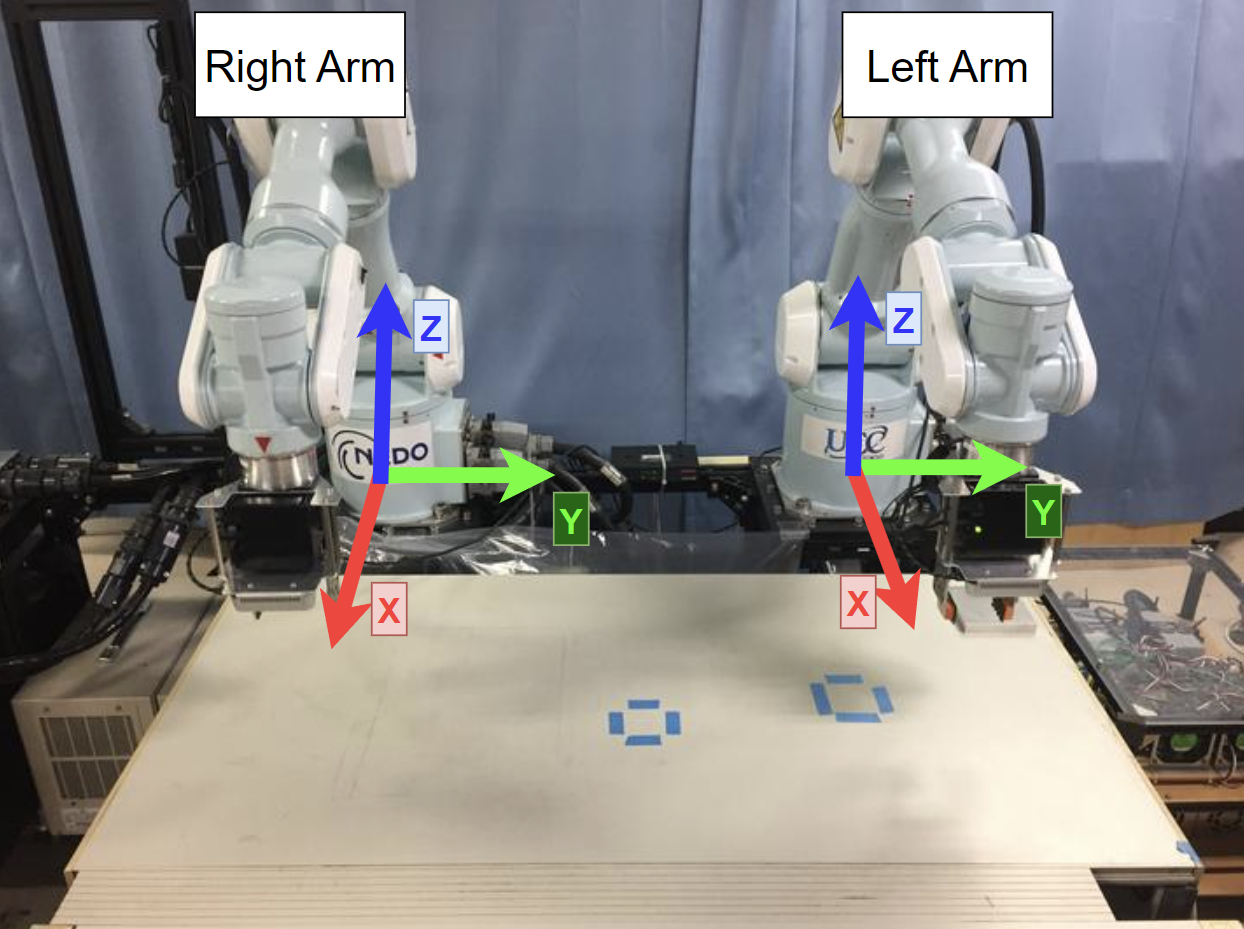
\includegraphics[width=0.8\linewidth]{fig/chp3/chp3_old_robot_coordinate.drawio.png}
    \caption{The coordinate system of PA10-7C.}
    \label{fig:system:robot-env-pa10}
\end{figure}

PA10-7Cを用いたロボットシステムでは，三菱重工製の7自由度マニピュレータPA10-7Cを2台用いた（図\ref{fig:system:robot-env-pa10}）．
両アームは卓上作業に適するよう床面から約700\,mmの高さに設置し，各アームのベース座標系の原点は各アームの底の中央に設定した．
この構成では，左右のアームを独立に制御しながら，片腕で対象物または道具を保持し，他方の腕で操作を実行する双腕協調作業を行う．

\paragraph{DENSO VS-050を用いた双腕ロボットシステム}

\begin{figure}[ht]
    \centering
    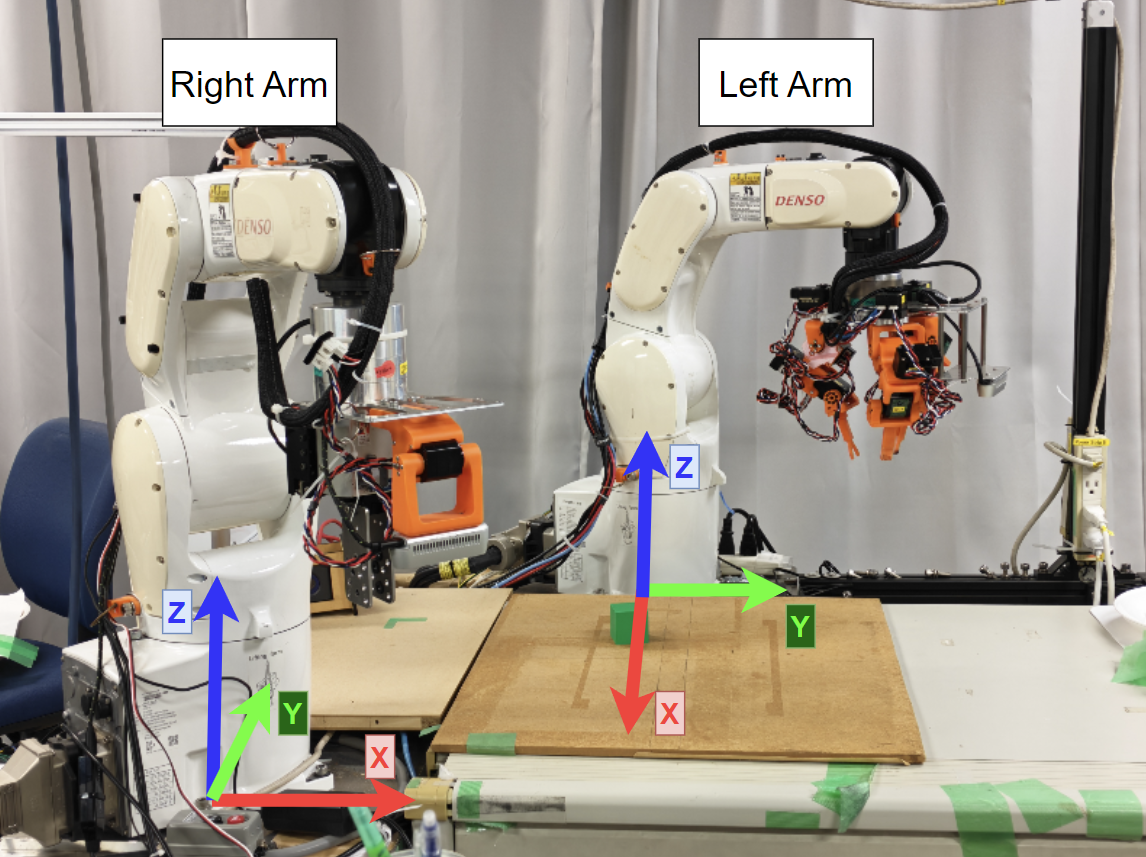
\includegraphics[width=0.8\linewidth]{fig/chp3/chp3_new_robot_coordinate.drawio.png}
    \caption{The coordinate system of DENSO VS-050.}
    \label{fig:system:robot-env-denso}
\end{figure}

DENSO VS-050を用いたロボットシステムでは，6軸の多関節ロボットVS-050を2台用いた（図\ref{fig:system:robot-env-denso}）．
VS-050は可搬質量4\,kg，位置繰り返し精度$\pm 0.02$\,mmの性能を有する．
本研究ではPA10-7Cの場合と同様に双腕構成として使用し，手先フランジ中心を基準としたツール座標系を定義した．
また，世界座標系は左アームのベース座標系に設定し，右アームで取得・計算される点群および操作点も同一の世界座標系上で扱えるようにした．

PA10-7CとDENSO VS-050では，アームの自由度や制御インタフェースが異なるため，ロボット固有の制御命令はそれぞれのロボットシステムに合わせて実装した．
一方，RGB-Dカメラから得られた点群を世界座標系へ変換し，3Dモデルとして後段の分析処理に渡すという処理の流れは共通である．

\subsection{力覚センサ}
\label{sec:system:hardware:force-sensor}
ロボットと対象物との接触を伴う操作を安定に実現するため，双腕の手首部には Leptrino 製の6軸力覚センサ PFS080YA501U6S を装備した（図\ref{fig:system:force-sensor-install}）．
このセンサはUSB経由で制御用PCに接続し，作業中に発生する力およびモーメントを計測する．

\begin{figure}[ht]
    \centering
    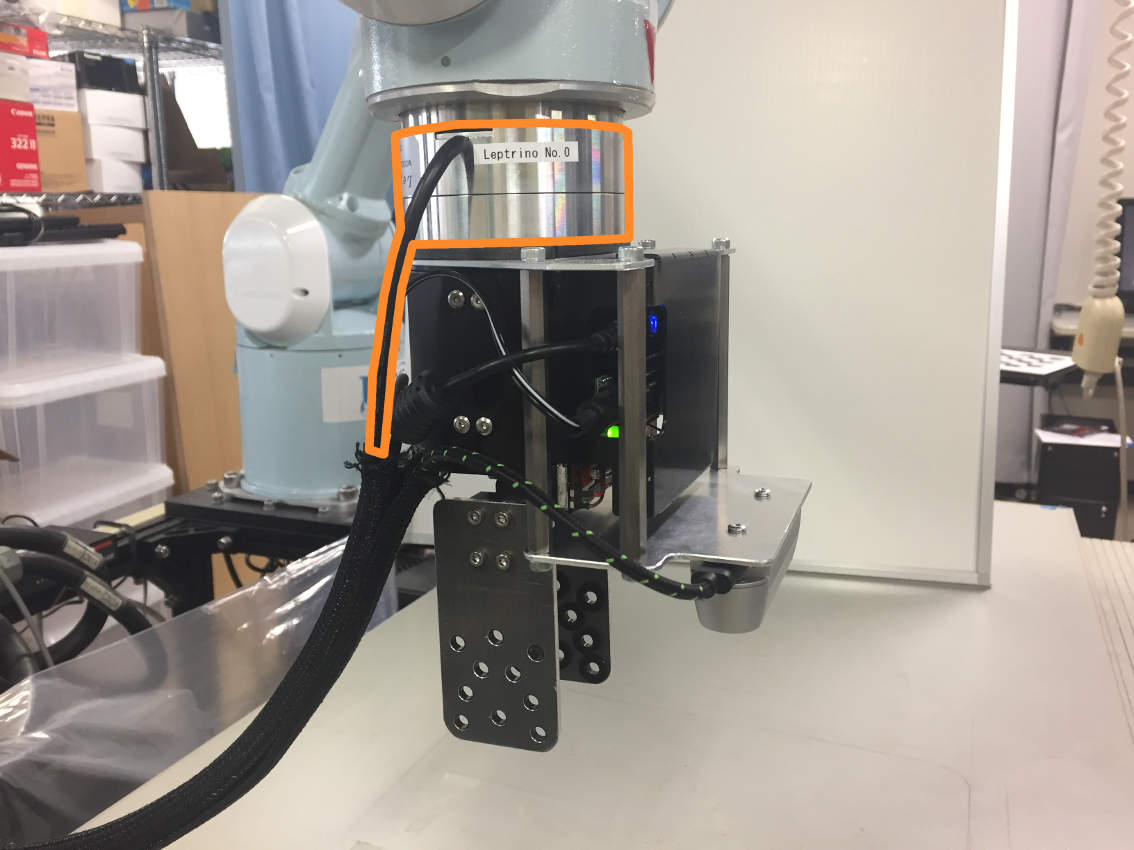
\includegraphics[width=.7\linewidth]{fig/chp3/ForceSensor.jpg}
    \caption{Six-axis Leptrino force sensor mounted on the wrist.}
    \label{fig:system:force-sensor-install}
\end{figure}

本センサの性能パラメータを表\ref{tab:system:force-sensor-spec}に示す．
データシートに基づき，本センサの力の分解能は以下の通り計算される：

\begin{equation}
\begin{split}
\text{分解能} &= \text{定格荷重} \times \text{分解能} \\
&= 500\;\mathrm{N} \times (1 / 4000) \\
&= 0.125\;\mathrm{N}
\end{split}
\end{equation}

% \begin{figure}[ht]
%     \centering
%     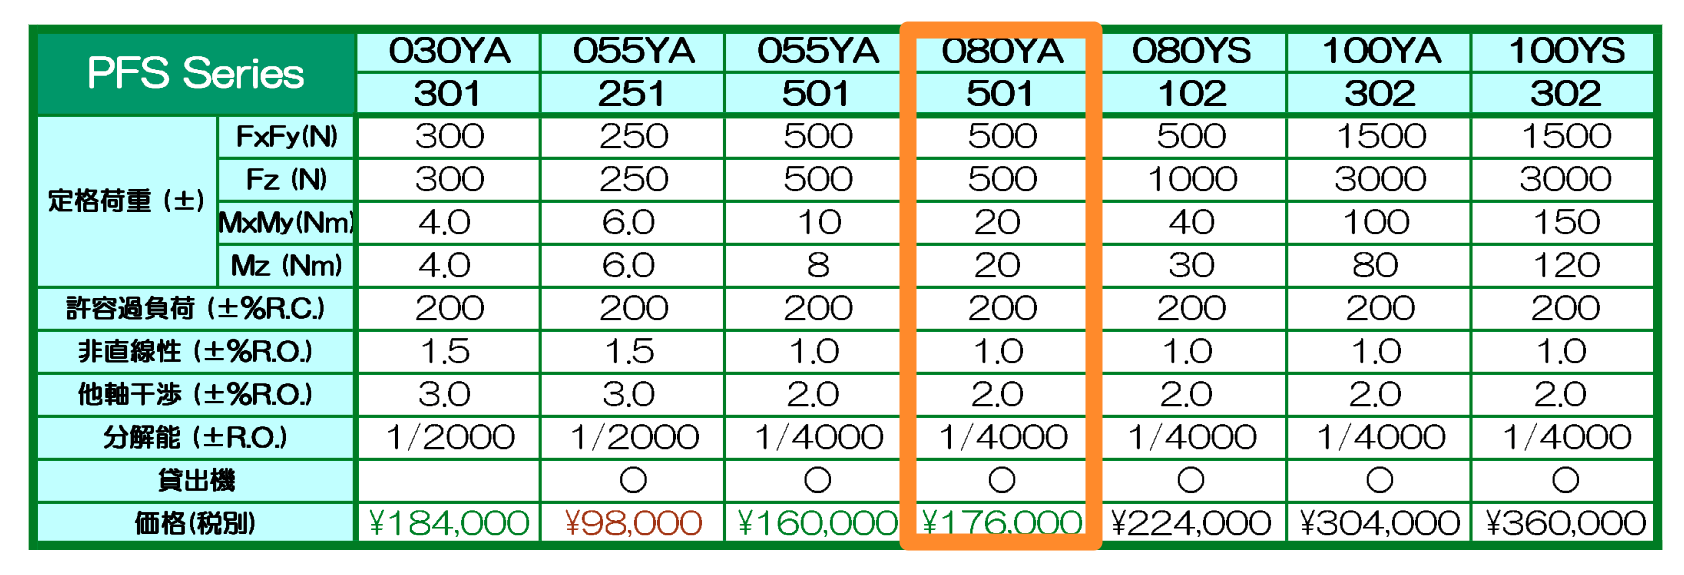
\includegraphics[width=1\linewidth]{fig/chp3/ForceSensor-performence.png}
%     \caption{Specification sheet of the PFS080YA501U6S.}
%     \label{fig:system:force-sensor-spec}
% \end{figure}
\begin{table}[ht]
  \centering
  \caption{Main specifications of the PFS080YA501U6S \cite{leptrino_6axis_force_sensor}.}
  \label{tab:system:force-sensor-spec}
  \begingroup
  \footnotesize
  \setlength{\tabcolsep}{4pt}
  \renewcommand{\arraystretch}{0.8}
  \begin{tabular}{@{}ll@{}}
    \toprule
    Item & Specification \\
    \midrule
    % Model & PFS080YA501U6 \\
    Rated force capacity ($F_x$, $F_y$, $F_z$) & $\pm 500$ N \\
    Rated moment capacity ($M_x$, $M_y$, $M_z$) & $\pm 20$ N$\cdot$m \\
    % Allowable overload & $\pm 200\%$ R.C. \\
    % Nonlinearity & $\pm 1.0\%$ R.O. \\
    % Inter-axis interference & $\pm 2.0\%$ R.O. \\
    Resolution & $1/4000$ \\
    \bottomrule
  \end{tabular}
  \endgroup
\end{table}

% 力覚情報は，特にツールと対象表面との接触が重要となる皮むき動作において有効であり，接触状態の確認および制御入力の設計に用いた．
% また，本論文では，3Dモデルに基づく幾何学的解析に加えて，接触に伴う力学的な情報も操作設計の一部として扱うため，力覚センサはそのための共通計測基盤として位置づけられる．
力覚情報は，皮むき動作では接触状態の監視と力フィードバック制御の入力として，把持研究では把持安定性の評価の補助情報として用いた．
このように，力覚センサは3Dモデルを補完する計測手段として，接触を伴うタスクにおいて重要な役割を担う．

\subsection{視覚センサ}
\label{sec:system:hardware:vision-sensor}

対象物および作業環境の3D情報取得には，Intel RealSense D435 を用いた．
\begin{revisionblock}
本センサはRGB画像と深度画像を同時に取得できるRGB-Dカメラである．
本研究では，軌道，把持候補，容積を計算するための三次元幾何に加え，皮むき済み領域の識別などに色情報も必要となるため，両者を同一装置，同一視点で取得できるRGB-D方式を採用した．
レーザスキャナ等は条件によってより高精度な距離計測が可能であるが，色情報を得る別カメラとセンサ間校正が必要になり，家庭用システムで重視される小型性，構成の簡潔さ，およびコストの面で不利となる．
一方，RGB-D方式にも，鏡面反射，透明・半透明物体，液面，遮蔽および距離条件による欠測・ノイズがある．
そこで，本研究では反射面を含めて常に安定に計測できるとは仮定せず，多視点計測，外れ値除去，および後述する精度評価を組み合わせ，対象範囲で利用可能な点群を得る．
\end{revisionblock}
図\ref{fig:system:robot-camera}のように，カメラは主としてグリッパ前面に取り付け，ロボットアームの動作により視点を変化させることで，複数視点から点群を取得した．
同時に異なる角度から点群を撮影する目的で，RealSense D435を両アームに取り付けた．

\begin{figure}[ht]
    \centering
    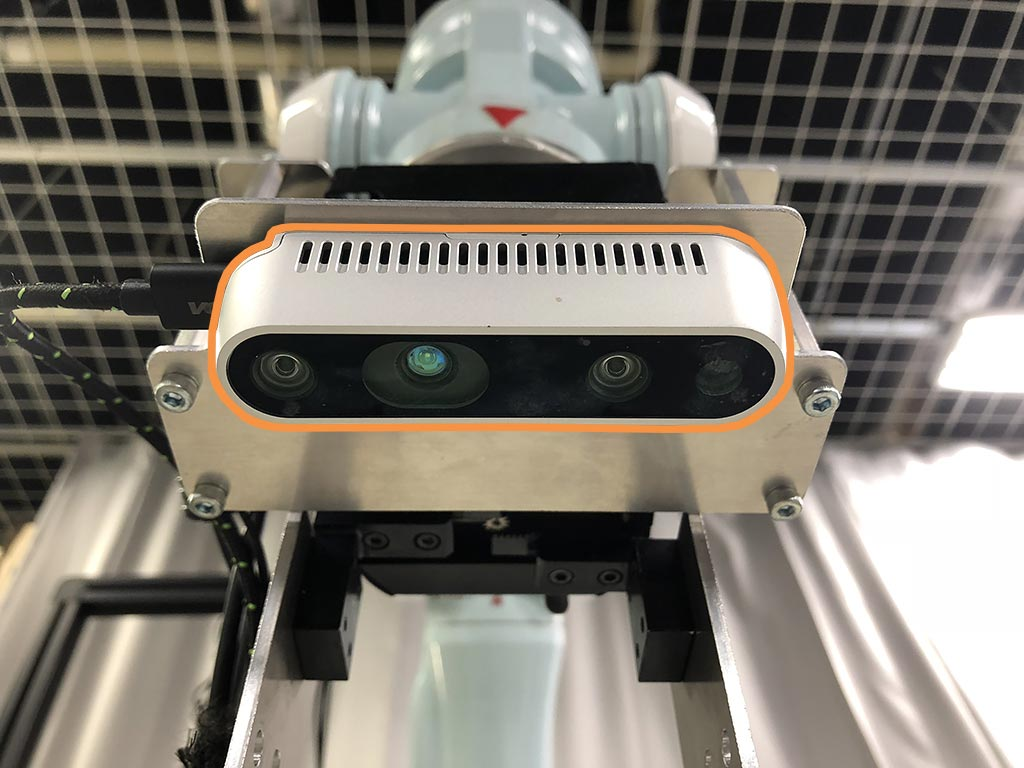
\includegraphics[width=.7\linewidth]{fig/chp3/Realsense.jpg}
    \caption{Intel RealSense D435 mounted on the wrist.}
    \label{fig:system:robot-camera}
\end{figure}

取得した点群は，各時刻におけるロボット姿勢とカメラの取り付け関係に基づいて世界座標系へ変換し，合成した3Dモデルとして利用する．
この3Dモデルは，注ぐ動作では容器内部形状の推定と容積計算に，皮むき動作では食材表面形状の取得とツール軌道生成に，安定把持では接触候補点の生成と把持安定性評価に用いられる．



\subsection{座標系定義とカメラキャリブレーション}
\label{sec:system:camera_calibration}

%%%%%
% \subsection{座標系定義とカメラキャリブレーション}
\label{sec:system:pointcloud:acquisition:calibration}

\paragraph{座標系の定義と接続関係}
\label{sec:system:hardware:coordinate-system}

本システムでは，RGB-Dカメラで取得した点群，ロボット手先の位置姿勢，
および各タスクにおけるツール先端位置を同一の基準で扱うため，複数の座標系を定義する．
各ロボットベース座標系の軸方向は，ロボット前方を$x$軸，
ロボットから見て左方向を$y$軸，鉛直上方を$z$軸とした．
回転の表現には$x$-$y$-$z$軸周りのオイラー角を用い，
各回転角度を$\alpha,\beta,\gamma$と表す．
正の回転方向は，各回転軸に対する右手系の正方向に従うものとする．

本論文では，以下の座標系を用いる．

\begin{enumerate}
  \item \textbf{ロボットベース座標系} $\Sigma_{B}$（Base）：
  各ロボットの基座中央を原点とする座標系である．
  双腕構成では，左腕のベース座標系を$\Sigma_{B_L}$，
  右腕のベース座標系を$\Sigma_{B_R}$と表す．
  各ロボットの関節角から得られる順運動学は，まず各ベース座標系を基準として計算される．

  \item \textbf{世界座標系} $\Sigma_{W}$（World）：
  本論文で扱う全タスクの共通基準座標系であり，
  左腕ロボットのベース座標系$\Sigma_{B_L}$と一致させる．
  すなわち，$\Sigma_W \equiv \Sigma_{B_L}$である．
  取得した点群，操作対象物，ツール先端位置，および左右腕の動作目標は，
  最終的にこの世界座標系上で記述する．

  \item \textbf{ロボット手先座標系} $\Sigma_{H}$（Hand）：
  ロボットアームの手首先端または手先フランジに固定された座標系であり，
  ロボットの移動指令およびツール座標系設定の基準となる．
  左腕と右腕を区別する場合は，それぞれ$\Sigma_{H_L}$，$\Sigma_{H_R}$と表す．

  \item \textbf{カメラ座標系} $\Sigma_{C}$（Camera）：
  RGB-Dカメラの光学中心を原点とし，
  カメラの光学軸を$z$軸とする座標系である．
  深度画像から復元された点群は，まずこの座標系で表される．

  \item \textbf{ツール座標系} $\Sigma_{T}$（Tool）：
  各タスクで使用するツールやエンドエフェクタの操作を容易にするため，
  ユーザが必要に応じて定義する座標系である．
  原点は，ピーラーの刃先，容器把持点，指先中心，包丁刃先など，
  作業において制御したい点に設定する．
  姿勢はツールの機能方向に合わせて定義し，
  手先座標系$\Sigma_H$に対する固定変換として与える．
\end{enumerate}

これらの座標系は，世界座標系$\Sigma_W$を基準として接続される．
左腕については，$\Sigma_W$と$\Sigma_{B_L}$が一致するため，
左腕手先の世界座標系における姿勢は順運動学から直接得られる．
一方，右腕については，右腕ベース座標系$\Sigma_{B_R}$から
左腕ベース座標系$\Sigma_{B_L}$への変換を介して，
右腕手先の姿勢を世界座標系へ変換する．

双腕ロボットの二つのベース座標系間の変換は，
同一位置に固定したChArUcoボードを左右のカメラから観測することで同定した．
これにより，左右のロボットで計算された手先位置，
左右のカメラで取得された点群，および各タスクの操作点を，
同一の世界座標系$\Sigma_W$上で扱うことができる．
% PA10-7Cを用いた構成では，両腕のベース座標系間の距離は$Y$軸方向に804\,mmであり，
% DENSO VS-050を用いた構成のベース配置については
% \ref{sec:system:configuration-changes:hardware}節で述べる．

手先座標系は，各ロボットの関節角と順運動学により，
親となるベース座標系に対する姿勢が得られる．
カメラ座標系は，カメラキャリブレーションにより，
手先座標系，ツール座標系，または1軸サーボカメラアームの関節座標系に対する
取り付け関係として決定される．
また，ツール座標系は，各タスクのツールやエンドエフェクタに応じてユーザが定義し，
手先座標系に対する固定変換として扱う．

手先に固定されたカメラで取得した点$\bm{p}$を同次座標で表すと，
カメラ座標系$\Sigma_C$から世界座標系$\Sigma_W$への変換は次式で記述される．

\begin{equation}
  {}^{W}\bm{p}
  =
  {}^{W}\bm{T}_{H}
  \cdot
  {}^{H}\bm{T}_{C}
  \cdot
  {}^{C}\bm{p}
  \label{eq:system:transform_chain}
\end{equation}

ここで，${}^{W}\bm{T}_{H}$は手先座標系から世界座標系への同次変換行列である．
左腕では順運動学により直接得られ，右腕ではベース間変換を含めて計算される．
${}^{H}\bm{T}_{C}$は手先座標系に対するカメラ座標系の取り付け位置姿勢，
${}^{C}\bm{p}$はカメラ座標系における点の位置ベクトルである．
なお，カメラがツールまたは1軸サーボカメラアームを介して取り付けられる場合には，
式\eqref{eq:system:transform_chain}中の${}^{H}\bm{T}_{C}$を，
該当する取り付け変換に置き換えて用いる．

同様に，ツール先端の姿勢は次式で表される．

\begin{equation}
  {}^{W}\bm{T}_{T}
  =
  {}^{W}\bm{T}_{H}
  \cdot
  {}^{H}\bm{T}_{T}
  \label{eq:system:tool_transform}
\end{equation}

ここで，${}^{H}\bm{T}_{T}$は各タスクで定義される
手先座標系からツール座標系への固定変換である．
ツール座標系を用いることで，ロボットの手先フランジではなく，
実際に作業を行うツール先端を目標位置・姿勢へ直接誘導できる．
例えば，ピーラーでは刃先位置，注ぎ作業では容器把持部または容器姿勢，
安定把持では指先接触点や包丁の刃先位置を基準として動作を記述できる．
PA10-7Cでは三菱重工が提供するPAライブラリを用いて手先の位置姿勢を制御するため，
ロボット手先に対するツール座標系$\Sigma_T$の位置・姿勢を
プログラム上で調整可能とした．
PA10-7Cにおけるツール座標系の設定例を図\ref{fig:system:tool-coordinate}に示す．

\begin{figure}[ht]
    \centering
    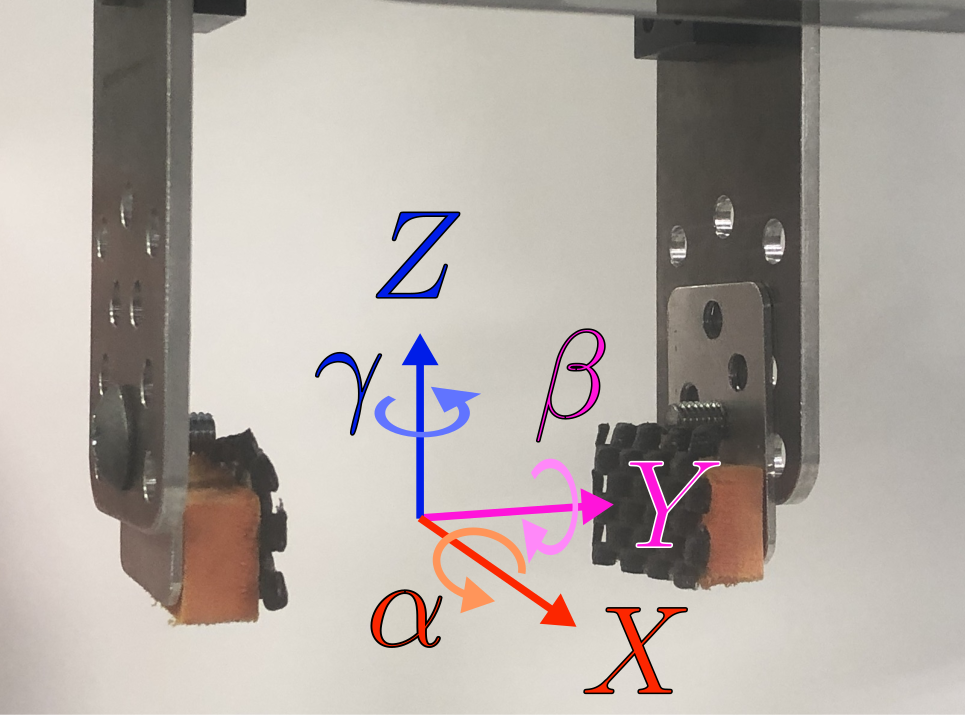
\includegraphics[width=0.7\linewidth]{fig/chp3/ToolCoordinate.png}
    \caption{Tool coordinate system.}
    \label{fig:system:tool-coordinate}
\end{figure}

\paragraph{カメラキャリブレーションと外部パラメータ}


RGB-Dカメラから取得した点群を多視点で合成するためには，
深度画像から復元された各点を，各撮影時のカメラ姿勢に基づいて
世界座標系へ変換する必要がある．
本研究では，カメラ内部パラメータ，手先座標系に対するカメラの取り付け位置姿勢，
左右アームのベース座標系間の変換，およびDENSO VS-050で用いた
1軸サーボカメラアームの角度依存変換を事前に同定した．

カメラ内部パラメータは，キャリブレーションボードを用いた通常の
カメラキャリブレーションにより取得し，深度画像からカメラ座標系の点群へ
逆投影する際に用いた．
以下では，多視点点群合成に直接関係する外部パラメータについて述べる．

\paragraph{ハンドアイキャリブレーション}
\label{sec:system:hand_eye}

手先に固定したカメラを用いる構成では，ロボット手先座標系 $\Sigma_H$ に対する
カメラ座標系 $\Sigma_C$ の固定変換 ${}^{H}\bm{T}_{C}$ を
ハンドアイキャリブレーションにより求めた．
具体的には，ChArUcoボードを作業空間内に静置し，ロボット手先を複数姿勢に
移動させながらボードを撮影した．
各画像から得られるボードとカメラの相対姿勢，およびロボットの順運動学から得られる
手先姿勢を用いて，OpenCVの
\texttt{calibrateRobotWorldHandEye} により
${}^{H}\bm{T}_{C}$ を推定した．
得られた変換は環境設定ファイルに保存し，実行時にはロボットの手先姿勢と合成して，
カメラ座標系で得られた点群を世界座標系へ変換する．

また，双腕ロボットでは左右アームのベース座標系を統一する必要がある．
本論文では左アームのベース座標系を世界座標系 $\Sigma_W$ として定義し，
同一のChArUcoボードを左右アームから観測することで，右アームのベース座標系
$\Sigma_{B_R}$ から左アームのベース座標系 $\Sigma_{B_L}$ への変換を求めた．
左右の観測から得られるボード姿勢をそれぞれ
${}^{B_L}\bm{T}_{\mathrm{cb}}$，
${}^{B_R}\bm{T}_{\mathrm{cb}}$ とすると，ベース座標系間の変換は次式で表される．

\begin{equation}
  {}^{B_L}\bm{T}_{B_R}
  =
  {}^{B_L}\bm{T}_{\mathrm{cb}}
  \left({}^{B_R}\bm{T}_{\mathrm{cb}}\right)^{-1}
  \label{eq:system:base_to_base}
\end{equation}

これにより，左右のカメラで取得した点群，および各アームで計算された操作点を，
同一の世界座標系上で扱うことが可能となる．

\paragraph{1軸サーボカメラアームのキャリブレーション}
\label{sec:system:servo_cam_calib}

\begin{figure}[ht]
  \centering
  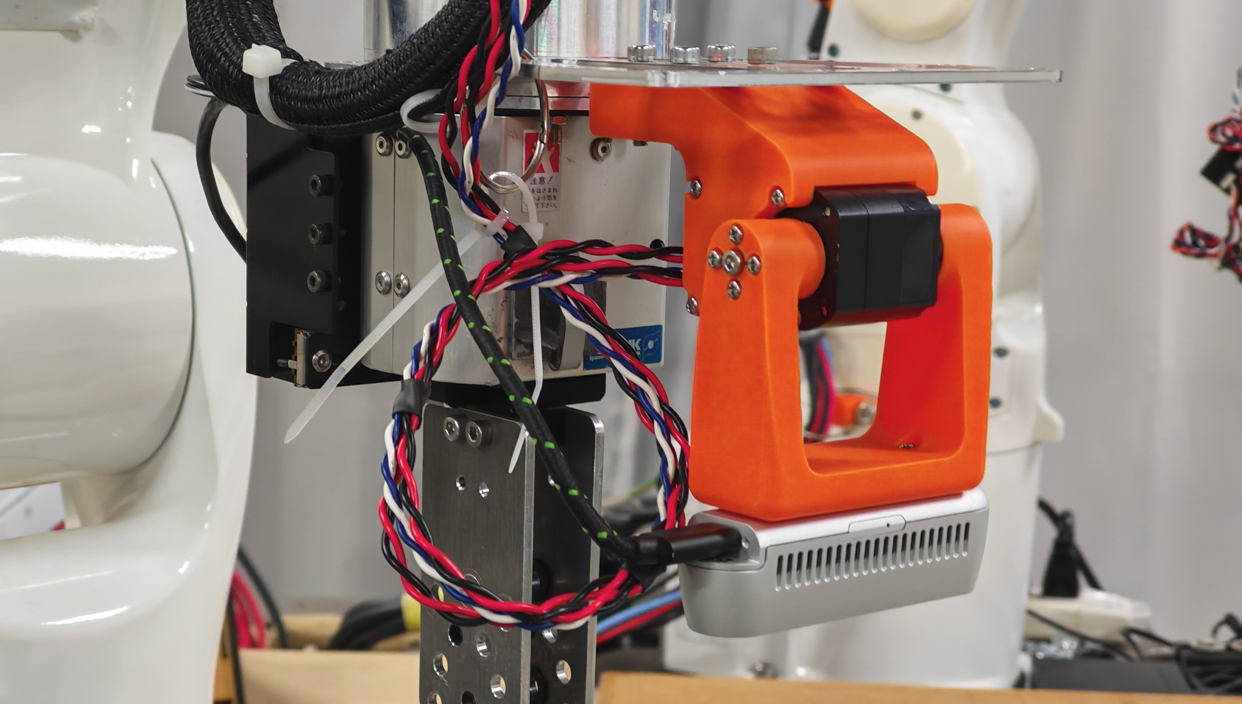
\includegraphics[width=.7\linewidth]{fig/chp3/chp3_new_robot_camera_arm.png}
  \caption{The camera arm for DENSO VS-050.}
  \label{fig:system:robot-camera-arm-denso}
\end{figure}

DENSO VS-050を用いたロボットシステムでは，ロボットの可動範囲の制約を補うため，
RGB-Dカメラを1軸サーボアームに取り付けた
（図\ref{fig:system:robot-camera-arm-denso}）．
このカメラアームはロボット手先に固定されているため，カメラ姿勢は手先座標系
$\Sigma_H$ を上位座標系として，サーボ角 $\theta$ に応じて変化する．
したがって，固定カメラ構成で用いた一定値の ${}^{H}\bm{T}_{C}$ ではなく，
角度依存の変換 ${}^{H}\bm{T}_{C}(\theta)$ を用いる．

本研究では，サーボカメラアームを1自由度の回転関節としてモデル化した．
手先座標系 $\Sigma_H$ からカメラ座標系 $\Sigma_C$ への変換は，
サーボ関節座標系 $\Sigma_J$ を介して次式で表される．

\begin{equation}
  {}^{H}\bm{T}_{C}(\theta)
  =
  {}^{H}\bm{T}_{J}
  \begin{bmatrix}
    R(\bm{a},\,\theta) & \bm{0} \\
    \bm{0}^{\top} & 1
  \end{bmatrix}
  {}^{J}\bm{T}_{C}
  \label{eq:system:servo_camera_model}
\end{equation}

ここで，$\bm{a}$ はサーボ関節座標系における回転軸，
$\theta$ はサーボ関節角である．
また，${}^{H}\bm{T}_{J}$ は手先座標系からサーボ関節座標系への固定変換，
${}^{J}\bm{T}_{C}$ はサーボ関節座標系からカメラ座標系への固定変換である．

これらのパラメータは，複数のサーボ角 $\theta$ においてChArUcoボードを観測し，
各角度で得られたカメラ姿勢と式\eqref{eq:system:servo_camera_model}の予測値が
最も一致するように，非線形最小二乗法により推定した．

実行時には，現在のサーボ角 $\theta$ から ${}^{H}\bm{T}_{C}(\theta)$ を計算し，
ロボットの順運動学により得られる手先姿勢と合成することで，
世界座標系におけるカメラ姿勢を求める．

\begin{equation}
  {}^{W}\bm{T}_{C}(\theta)
  =
  {}^{W}\bm{T}_{H}
  {}^{H}\bm{T}_{C}(\theta)
  \label{eq:system:world_camera_servo}
\end{equation}

以上のキャリブレーションにより，固定カメラ構成および1軸サーボカメラアーム構成の
いずれにおいても，RGB-Dカメラで取得した点群を世界座標系へ変換し，
多視点点群として合成できる．




\subsection{エンドエフェクタ設計}
\label{sec:system:hardware:end-effector}

\subsubsection{平行グリッパ}
\label{sec:system:hardware:parallel-gripper}
力覚センサの先端には，三菱電機製の平行グリッパ1E-HM01 HANDを取り付けた（図\ref{fig:system:parallel-gripper}）．
本グリッパの指先に取り付けられたアルミ板には，様々な姿勢でツールを装着できるように多数の穴が設けられており，各研究の要件に応じてエンドエフェクタを交換可能な構造となっている．

\begin{figure}[ht]
    \centering
    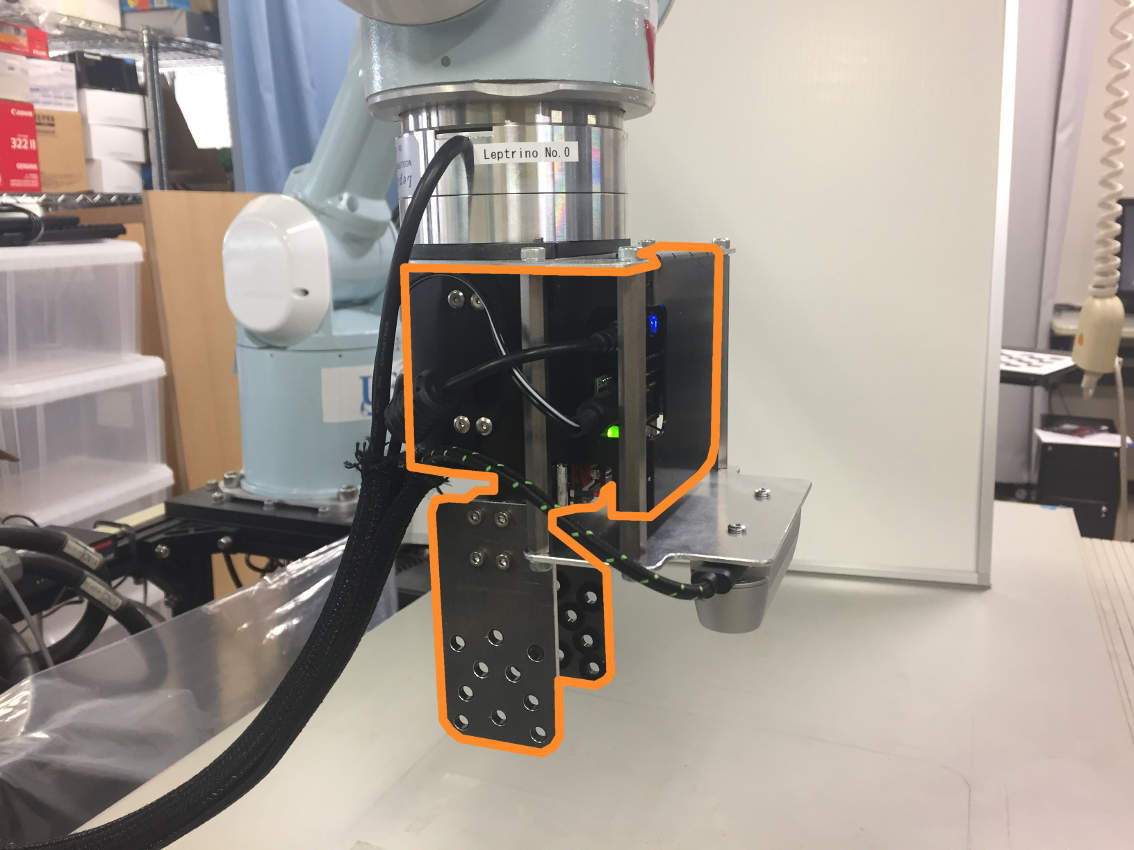
\includegraphics[width=.7\linewidth]{fig/chp3/Gripper.jpg}
    \caption{Parallel gripper indicated by the orange frame.}
    \label{fig:system:parallel-gripper}
\end{figure}

本論文では，この平行グリッパを，タスクに応じたエンドエフェクタを取り付けるための共通インタフェースとして用いた．
注ぎ用エンドエフェクタでは，指先アルミ板に容器把持用の接触部を取り付け，容器の縁部または外周部を把持した．
皮むき用エンドエフェクタでは，ピーラー固定部および食材固定用の$V$字溝部を同じ取付穴列に固定し，道具先端および食材固定位置を再現性よく設定した．
安定把持用エンドエフェクタでは，右腕側の平行グリッパを包丁固定用の高剛性把持部として利用し，左腕側は食材表面への接触点を柔軟に選択するため指型ハンドに置き換えた．


\subsubsection{皮むき用エンドエフェクタ}
\label{sec:system:hardware:peeling-end-effector}
皮むき動作では，片方の腕でピーラーを操作し，もう片方の腕で食材を固定する必要がある．
このため，両アームとも平行グリッパを基盤としつつ，役割に応じて異なるエンドエフェクタを装着した．

ツール側のエンドエフェクタ（図\ref{fig:system:peeling-end-effector-peeler}）としては，ピーラーをロボット手先へ固定するためのパーツを設計した．
このパーツにより，ピーラーの刃先位置と姿勢をツール座標系として明確に定義でき，食材表面形状に基づいて生成した軌道に従って刃先を安定に移動させることが可能となる．

\begin{figure}[ht]
    \centering
    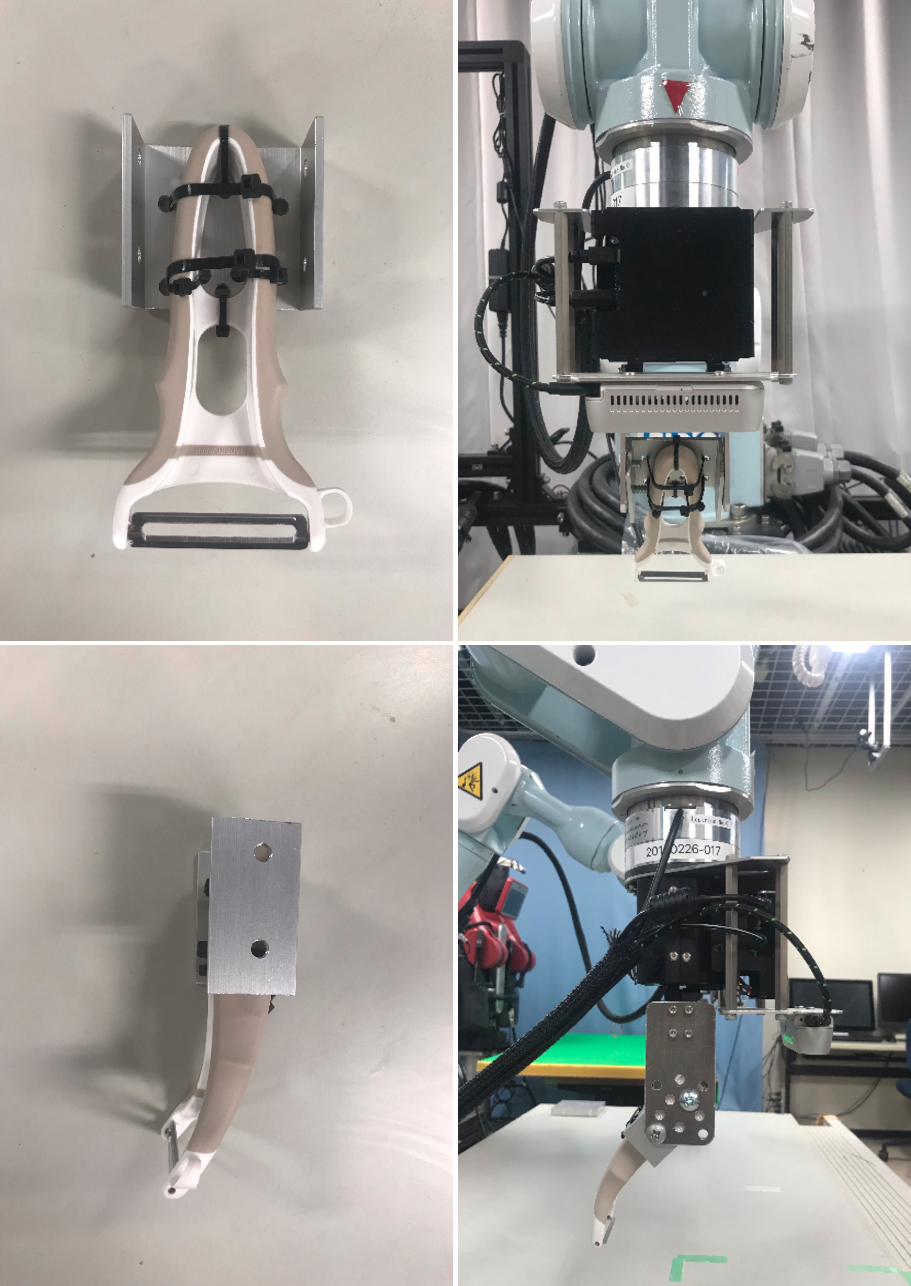
\includegraphics[width=.7\linewidth]{fig/chp3/PeelingEndeffector-2.pdf}
    \caption{Peeler-side end effector for the peeling task.}
    \label{fig:system:peeling-end-effector-peeler}
\end{figure}

食材固定側のエンドエフェクタとしては，食材に刺した串を安定に固定するための専用ぱパーツを用いた．
細長い串は通常の平行グリッパでは毎回同じ位置に保持することが難しいため，$V$字溝を有する把持部を設け，串が一定位置に自然に収まるように設計した（図\ref{fig:system:peeling-end-effector-food}）．
これにより，食材の姿勢再現性が向上し，皮むき軌道の安定な実行が可能となる．

\begin{figure}[ht]
    \centering
    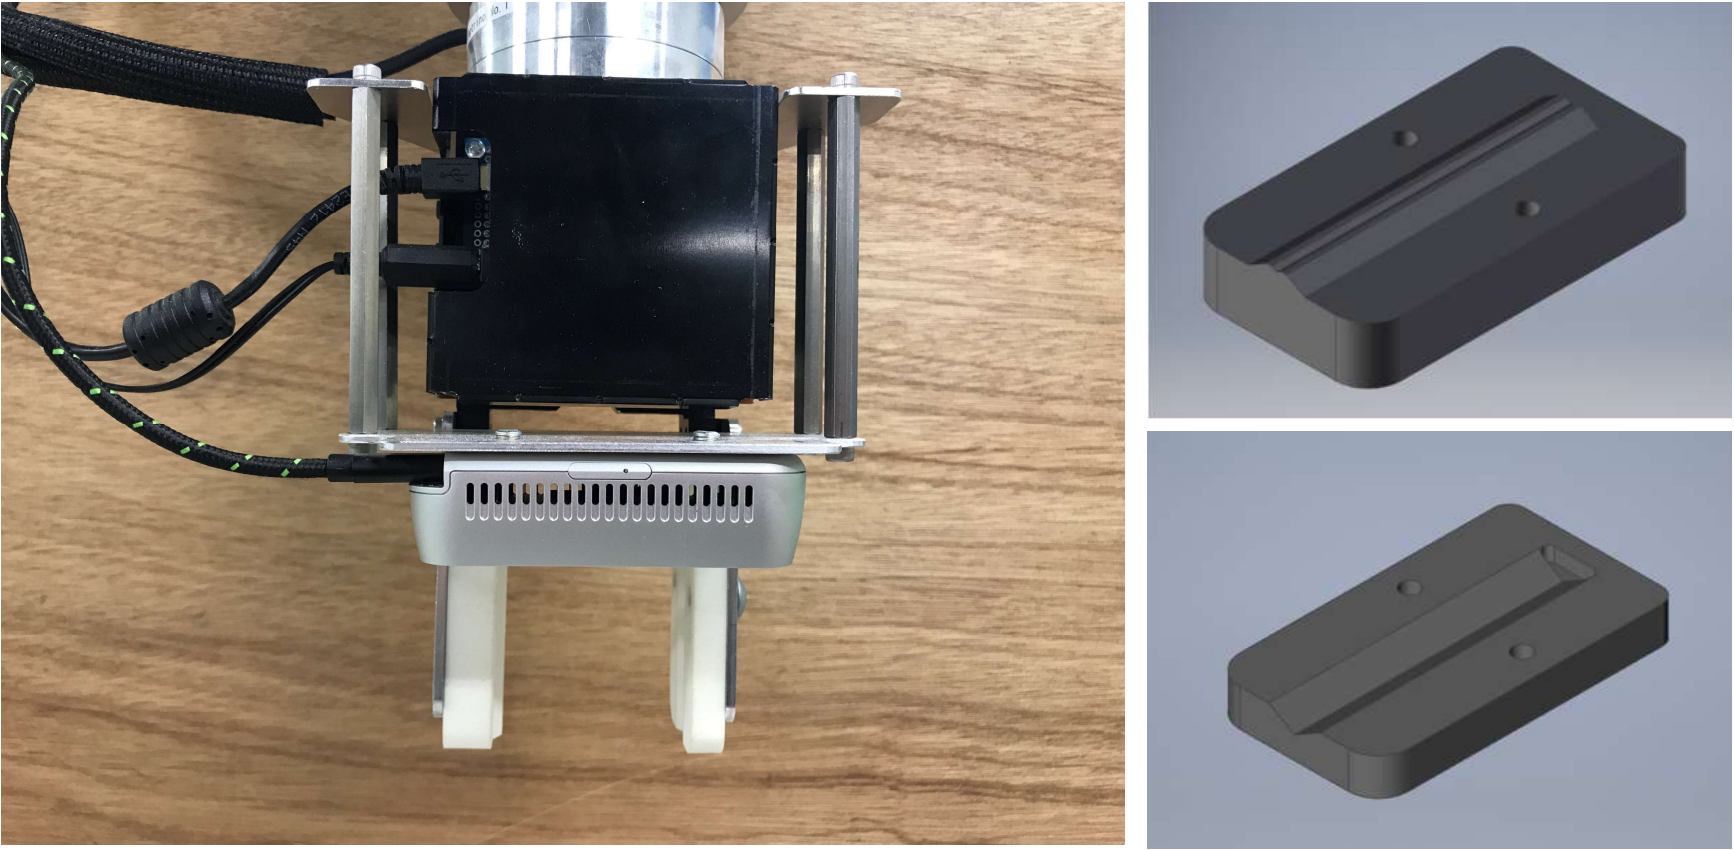
\includegraphics[width=.5\linewidth]{fig/chp3/PeelingEndeffector-1.png}
    \caption{Food-fixation end effector for the peeling task.}
    \label{fig:system:peeling-end-effector-food}
\end{figure}

\subsubsection{注ぎ用エンドエフェクタ}
\label{sec:system:hardware:pouring-end-effector}
注ぐ動作では，各種容器を安定に把持し，必要に応じて持ち上げ，傾ける必要がある．
そこで，平行グリッパを基盤とし，その指先アルミ板に容器把持用のエンドエフェクタを取り付けた．
本研究では，対象容器の形状差に対応するため，2種類のエンドエフェクタを用いた．

第1のエンドエフェクタ（図\ref{fig:system:pouring-end-effector-1}）は，ボウルやカップのように開口縁を有する容器を対象としたものである．
平行グリッパの開口幅（最大10\,cm）のみでは把持が困難な場合を想定し，容器本体ではなく縁部を把持できるように設計した．
また，把持時の摩擦力を高めるため，接触面には小型のスポンジを取り付けた．

\begin{figure}[ht]
    \centering
    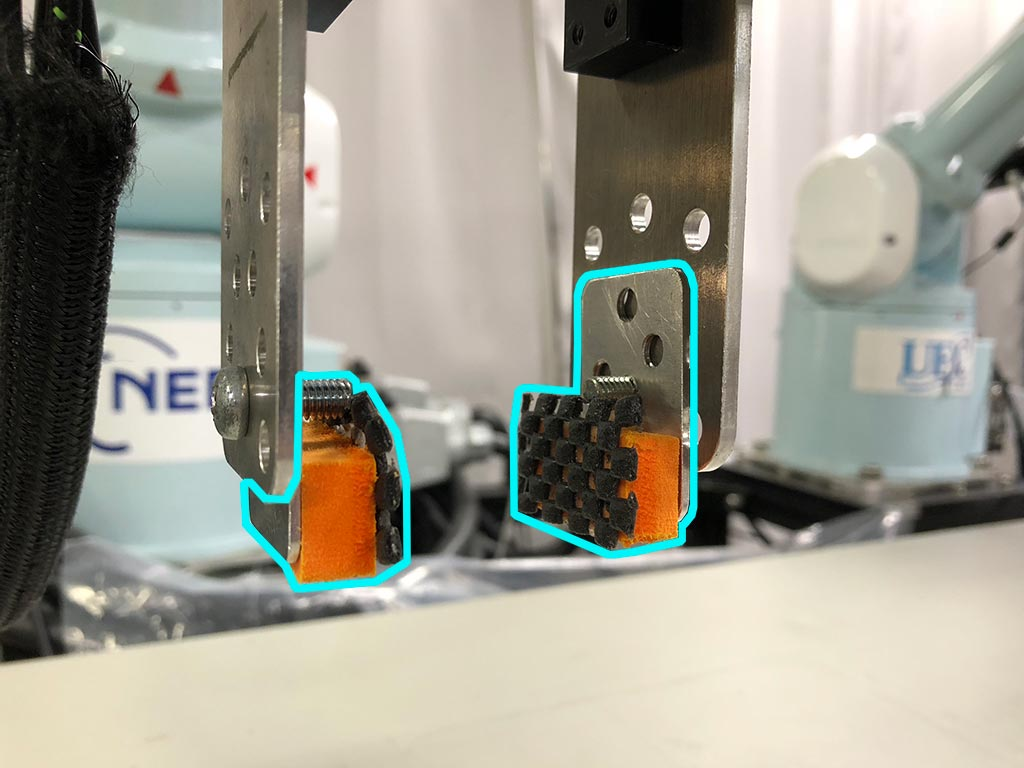
\includegraphics[width=.7\linewidth]{fig/chp3/PourEndFactor-1.jpg}
    \caption{End effector 1 for the pouring task.}
    \label{fig:system:pouring-end-effector-1}
\end{figure}

第2のエンドエフェクタ（図\ref{fig:system:pouring-end-effector-2}）は，外形寸法が比較的小さく，グリッパ開口幅内に収まる容器を確実に把持することを目的としたものである．
こちらも把持安定性向上のため，接触面に薄いスポンジを取り付けた．
このように，注ぐ動作におけるエンドエフェクタ設計では，容器形状の多様性に対して，把持を切り替えられることを重視した．

\begin{figure}[ht]
    \centering
    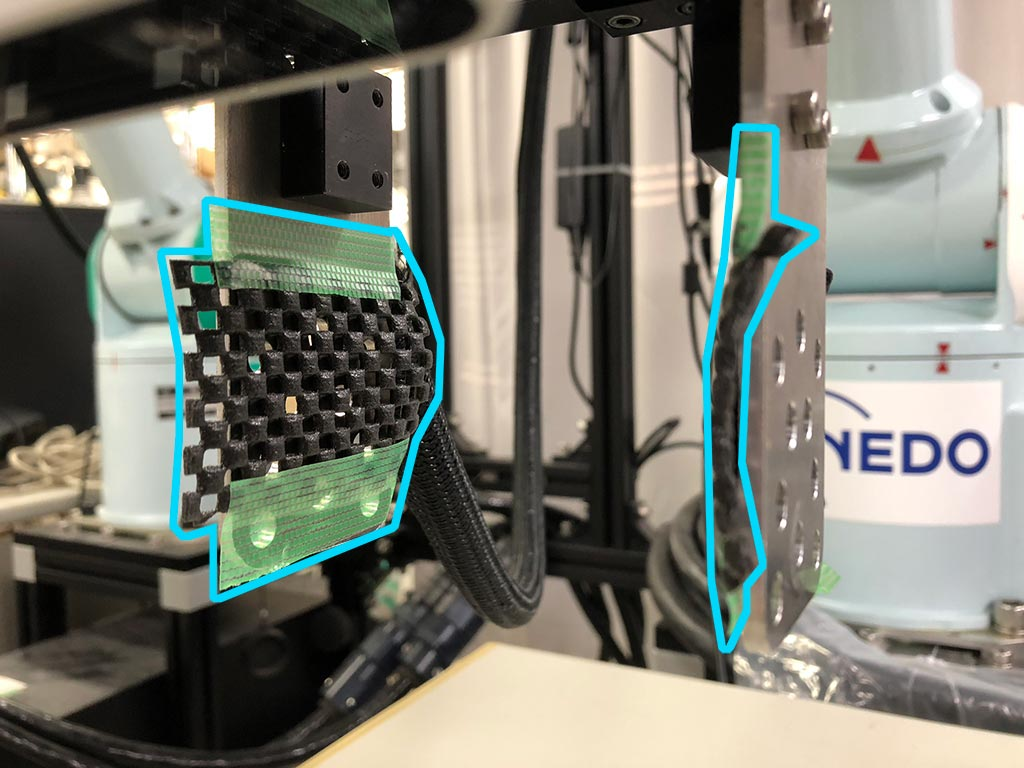
\includegraphics[width=.7\linewidth]{fig/chp3/PourEndFactor-2.jpg}
    \caption{End effector 2 for the pouring task.}
    \label{fig:system:pouring-end-effector-2}
\end{figure}

\subsubsection{安定把持用エンドエフェクタ}
\label{sec:system:hardware:holding-end-effector}
安定把持の研究では，左腕に食材把持用の指型ハンドを，右腕に包丁固定用の高把持力平行グリッパを装着した．
右アーム側の平行グリッパは，包丁をロボットへ剛結合することを目的としており，切断するときに発生する外力を安定に伝達できるようにした．
左アーム側では，食材形状に応じて接触点を柔軟に選択できることが重要であるため，多関節の指型ハンドを用いた．

食材把持用ハンドとしては，3軸2指のサーボハンドを用いた（図\ref{fig:system:finger-hand}）．
各指には FUTABAのサーボ RS405CB を使用し，最大トルクは48.0\,$\mathrm{kgf \cdot cm}$，角度分解能は0.1\,degである．
各指の関節構成は $z$-$y$-$y$-tip とし，指先位置を制御するために，ヤコビアンに基づく指関節のみの逆運動学を用いた．
この構成により，食材表面上に生成した候補接触点へ指先を誘導し，把持安定性の評価に基づいて適切な接触配置を実現できる．
\revise{指先は把持安定性の計算で仮定する点接触に近づけるため，食材に対する接触面を小さくした．また，包丁軌道と干渉せずに食材上面・側面の候補点へ届く指長と関節配置を採用し，カメラ観測時には指同士および指と食材による遮蔽が固定化しないよう，対象の提示姿勢を変更できる構成とした．}

\begin{figure}[ht]
    \centering
    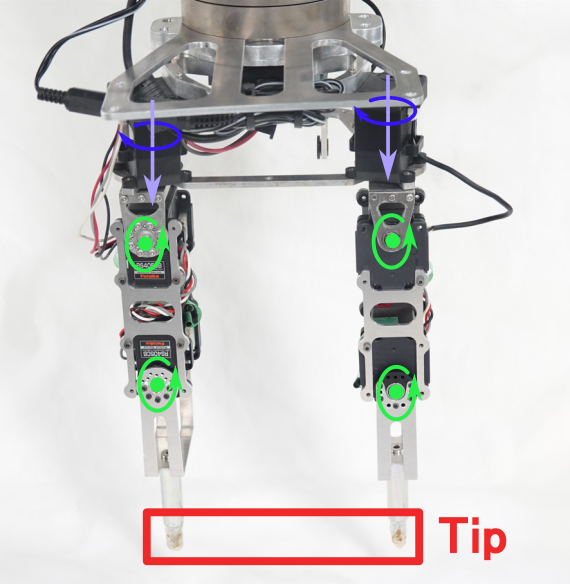
\includegraphics[width=.5\linewidth]{fig/chp3/ICRA_RobotHand.png}
    \caption{Finger hand used for holding.}
    \label{fig:system:finger-hand}
\end{figure}

このように，切断する時に把持におけるエンドエフェクタ設計では，包丁側には高剛性な固定機構を，食材側には形状適応性を有する多指ハンドを使用することで，切断時の外力と把持安定性の両立を図った．

% \subsection{座標系定義}
% \label{sec:system:hardware:coordinate-system}

% 各軸の向きはロボット前方を$x$軸，ロボットから見て左方向を$y$軸，鉛直上方を$z$軸とした．

% 双腕共同作業を統一的に記述するため，世界座標系を定義した．
% 世界座標系の原点は左アームのベース座標系と一致させ，各軸の向きも左アームのベース座標系と同様に設定した．
% 回転の表現には$x$-$y$-$z$軸周りのオイラー角を用い，各回転角度を$\alpha,\beta,\gamma$と表す．プラス回転方向は各回転軸に対して逆時計回りとした．

% また，各アームがお互いの動作を妨害せずに共同作業を可能とするため，両アームのベース座標系間の距離を$Y$軸方向に804\,mmとした．
% % Relative base transforms:
% % robot.denso.middle.base -> robot.denso.right.base (XYZABC, ABC in deg, Euler order XYZ):
% %   [0.433713, 0.759744, 0.064421, 1.607230, -0.778746, -92.196446]
% % robot.denso.right.base -> robot.denso.middle.base (XYZABC, ABC in deg, Euler order XYZ):
% %   [0.777336, -0.404764, -0.037188, -0.716564, -1.635894, 92.197139]

% \begin{figure}[ht]
%     \centering
%     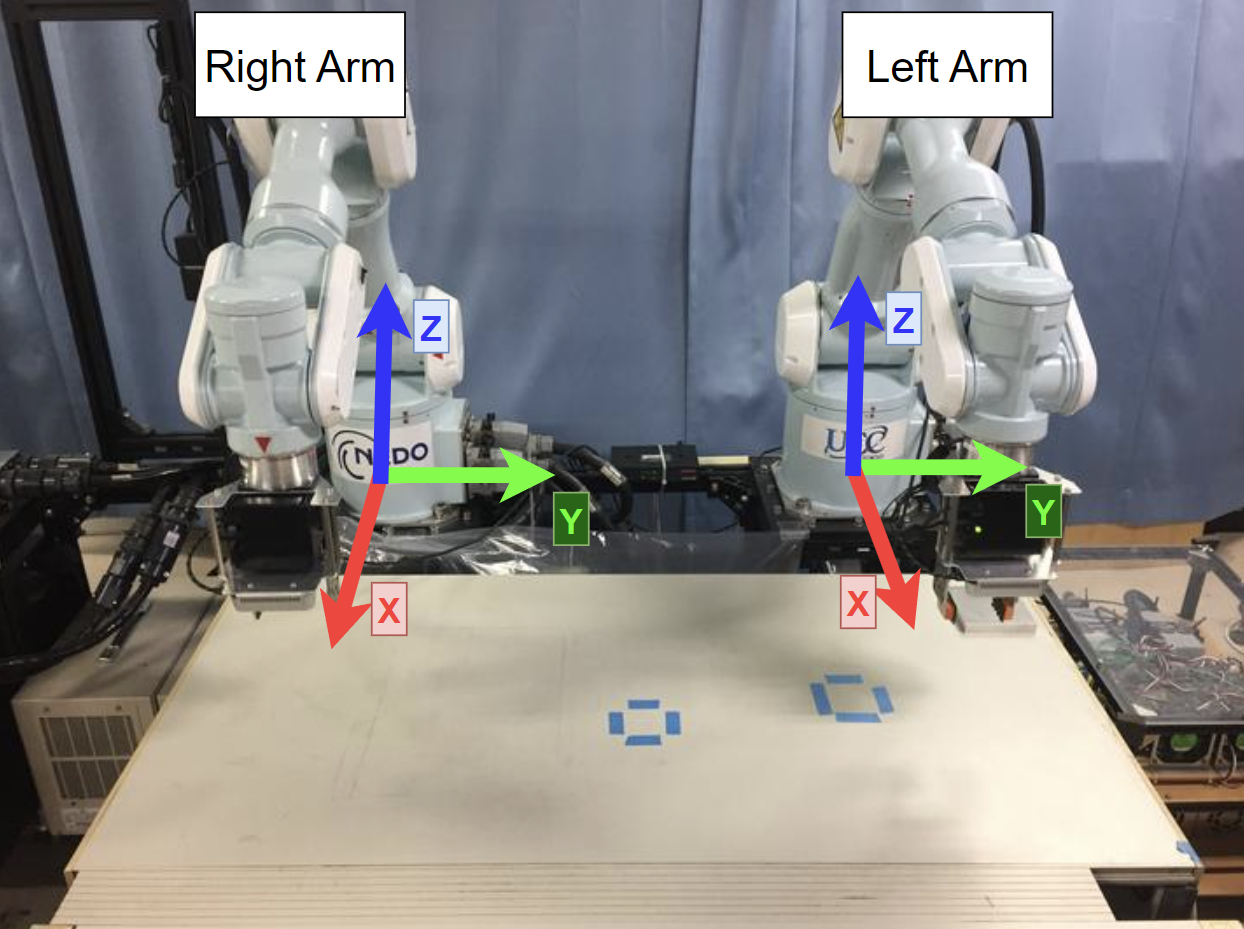
\includegraphics[width=0.8\linewidth]{fig/chp3/chp3_old_robot_coordinate.drawio.png}
%     \caption{The coordinate system of PA10-7C.}
%     \label{fig:system:robot-env-pa10}
% \end{figure}
% \begin{figure}[ht]
%     \centering
%     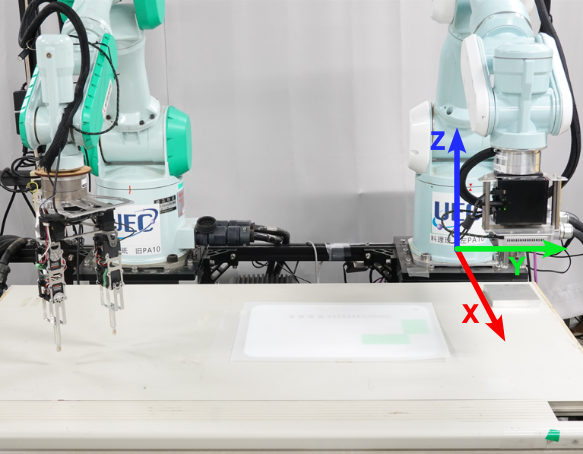
\includegraphics[width=.8\linewidth]{fig/chp3/ICRA_RobotEnv.png}
%     \caption{The coordinate system of PA10-7C. Right side robot is called [Left Arm]}
%     \label{fig:system:robot-env-pa10-alternative}
% \end{figure}
% \begin{figure}[ht]
%     \centering
%     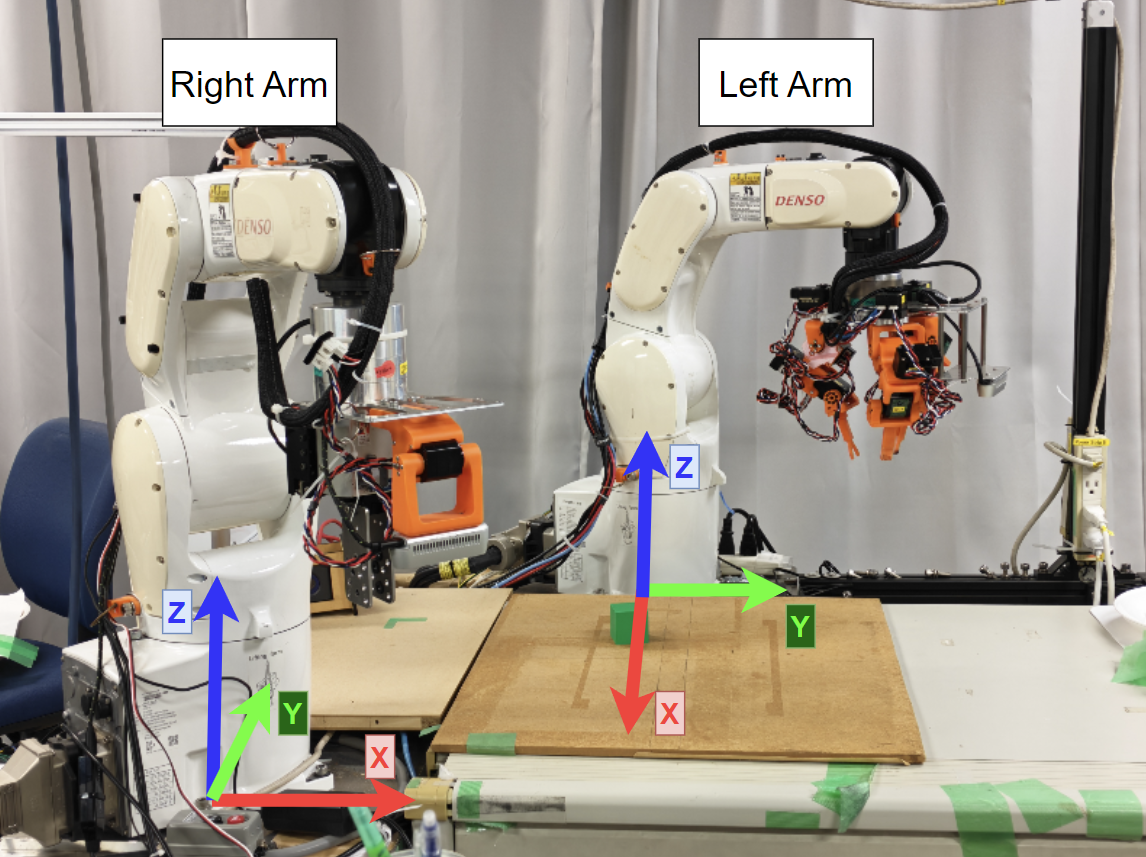
\includegraphics[width=.8\linewidth]{fig/chp3/chp3_new_robot_coordinate.drawio.png}
%     \caption{The coordinate system of DENSO VS-050.}
%     \label{fig:system:robot-env-denso-alternative}
% \end{figure}

% \paragraph{ツール座標系}

% ツール座標系は，ロボットが操作する道具の座標系である．
% 道具を目標の位置・姿勢へ誘導する際，ロボットの手先座標系を直接制御するよりも，道具先端に設定した座標系を制御するほうが直感的かつ高精度な動作記述が可能となる．

% PA10-7Cでは三菱重工が提供するPAライブラリを用いて手先の位置姿勢を制御する．
% 本研究では，ロボット手先にツールを装着した状態で各種作業を実行するため，以下のようにツール座標系を定義した．
% PA10手先座標系の原点は手先フランジの中心に位置し，姿勢はベース座標系に対して$Y$軸周りに180度回転させた姿勢である．
% ツール座標系の原点は装着したツールの中心（ピーラーであれば刃先，把持用エンドエフェクタであれば指先中心）に設定し，姿勢はPA10手先座標系から$Y$軸周りに180度回転させた姿勢，すなわちベース座標系と同一方向となるように定義した（図\ref{fig:system:tool-coordinate}）．
% 各種ツールに対応するため，ツール座標系の位置・姿勢はプログラム上で調整可能とした．

% \begin{figure}[ht]
%     \centering
%     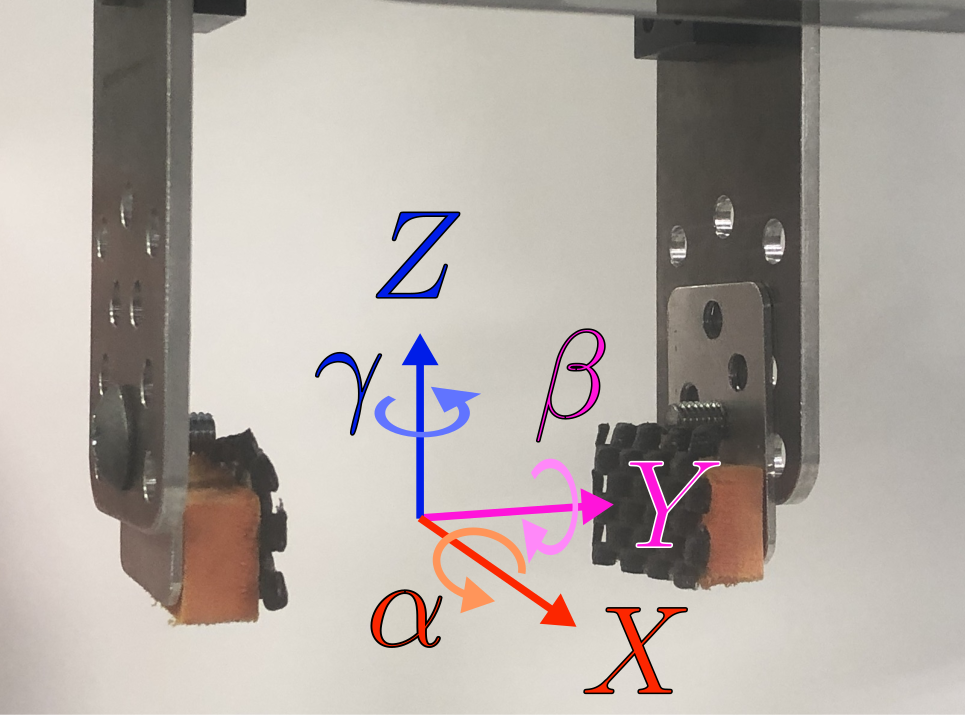
\includegraphics[width=0.7\linewidth]{fig/chp3/ToolCoordinate.png}
%     \caption{Tool coordinate system.}
%     \label{fig:system:tool-coordinate}
% \end{figure}

\section{システム構成：ソフトウェア}
\label{sec:system:software}

本研究を構成する三つの研究では，実施時期や要件の変化に伴い，ソフトウェア構成に段階的な変更が生じた．
しかし，点群処理アルゴリズムの本質（処理順番・パラメータ・出力仕様）は全研究で一貫している．
本節では，主に注ぐ・皮むきの研究で用いたOpenRTMベースのRTC統合アーキテクチャについて述べ，最後の把持の研究におけるソフトウェア構成の変更点を整理する．

\subsection{使用ライブラリ}
\label{sec:system:software:libraries}

\paragraph{librealsense}

librealsenseはIntel社がRealSenseシリーズのカメラを操作するために提供するクロスプラットフォームSDKである．
C++のほか，Python，MATLABなど複数のプログラミング言語に対応しており，PCLやOpenCV等のライブラリへのデータ受け渡しも容易である．
本ライブラリは，カメラに搭載された各種センサのデータ取得に加え，深度画像から点群データへの変換，カラー画像と深度画像の合成などのデータ処理機能を提供する．
本研究ではlibrealsense 2.11を用いた．

\paragraph{PCL（Point Cloud Library）}

\label{sec:system:software:pcl}

PCL（Point Cloud Library）は2次元・3次元の点群データを処理するためのオープンソースライブラリである\cite{PCL}．
フィルタリング，特徴量抽出，点群位置合わせ（Registration），近傍探索（KD-Tree），セグメンテーション，可視化など，点群処理に必要な機能がモジュール化されており，最新の研究手法を実装可能な拡張性を有する．
本研究ではPCL 1.8.0を用い，本章後半で述べる点群処理パイプラインの実装基盤とした．

\subsection{OpenRTMに基づくソフトウェアフレームワーク}
\label{sec:system:software:openrtm}
本研究では，RT-Middlewareの実装のひとつであるOpenRTM-aist\cite{RTM-aist}を用いてコンポーネント指向のロボット操作システムを構築した．
各ハードウェアをRT-Component（ハードウェアを操作するための独立プログラム，以下RTCとよぶ）として作成し，RTC-handle\cite{rtc_handle}を用いてこれらを接続することで，システム全体を統括した．
Pythonのメインスクリプトから関数をコールすることで，RTC-handleを介して各RTCに指令を送る構成とした．

\paragraph{システム全体の接続構成}

図\ref{fig:system:overall-connection-architecture}にシステム全体の接続構成を示す．
図のPA10 PCはロボット制御に特化した専用PCであり，その他の処理は共通PC上で実行される．

% TODO:这软件张图需要修复
\begin{figure}[ht]
    \centering
    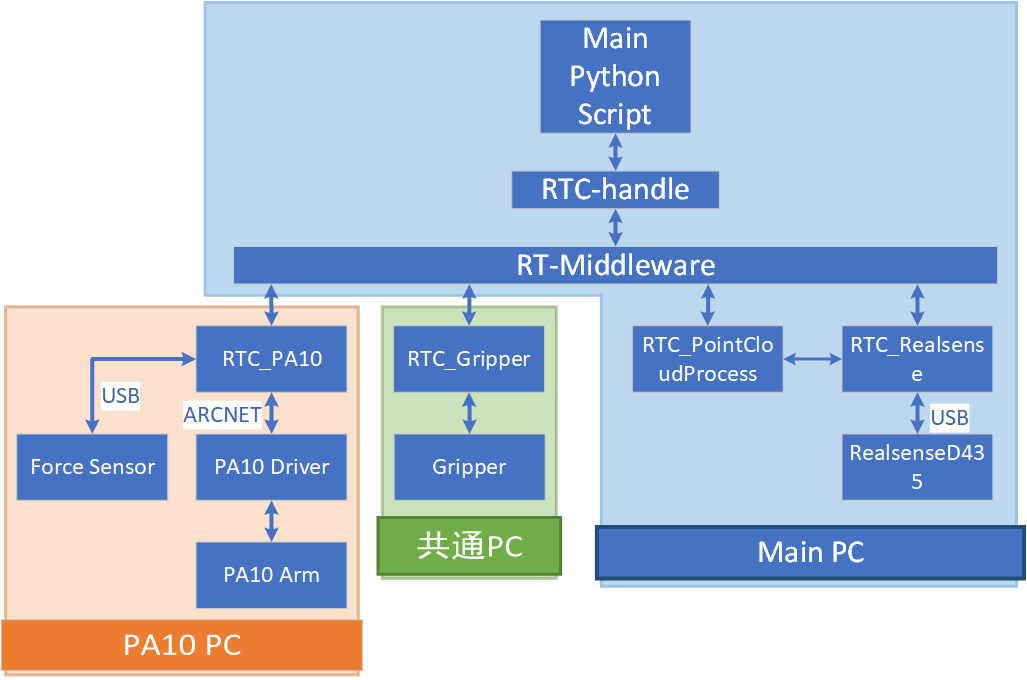
\includegraphics[width=0.9\linewidth]{fig/chp3/AllConnection.png}
    \caption{Overall connection architecture.}
    \label{fig:system:overall-connection-architecture}
\end{figure}

\paragraph{RTC\_PA10}

RTC\_PA10はPA10を操作するためのRTCである．
このRTCは専用PC（図\ref{fig:system:overall-connection-architecture}のPA10 PC）上で常時実行され，三菱重工が提供するPAライブラリを用いてARCNET経由でPA10のドライバと通信し，PA10ロボットを制御する．
リアルタイムの力のフィードバック制御を実現するため，力覚センサの操作メソッドも本RTCに組み込まれている．
RTC\_PA10のポート構成を図\ref{fig:system:rtc-pa10}に示す．

\begin{figure}[ht]
    \centering
    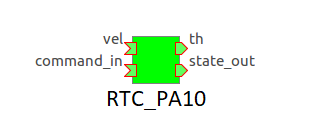
\includegraphics[width=0.4\linewidth]{fig/chp3/PA10Diag.png}
    \caption{Port configuration of RTC\_PA10.}
    \label{fig:system:rtc-pa10}
\end{figure}

\paragraph{RTC\_Gripper}

RTC\_Gripperは手先のグリッパを制御するためのRTCであり，グリッパの開閉動作を制御する．
保守性を考慮し，各腕のグリッパ用RTCはPA10 PC上ではなく，共通PC上で実行する構成とした．
RTC\_Gripperのポート構成を図\ref{fig:system:rtc-gripper}に示す．

\begin{figure}[ht]
    \centering
    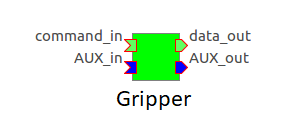
\includegraphics[width=0.4\linewidth]{fig/chp3/GripperDiag.png}
    \caption{Port configuration of RTC\_Gripper.}
    \label{fig:system:rtc-gripper}
\end{figure}

\paragraph{RTC\_Realsense}

RTC\_Realsenseは，librealsenseを用いてRealSense D435からカラー画像，赤外線画像，深度画像を取得し，RTC\_PointCloudProcessに送信するためのRTCである．
センサから取得したデータをRTCのデータ型に変換して出力するほか，深度画像から点群への変換，カラー画像の点群へのマッピング，深度画像のノイズ（librealsenseの内蔵フィルタ機能によるもので，\ref{sec:system:pointcloud:processing:pipeline}節で述べる点群処理パイプラインとは独立した前処理である）処理の各機能をRTC内に実装した．

データ処理とセンサ読込の速度差を吸収するため，各データチャネル（カラー，赤外線2系統，深度）にキューを設置した．
キューは常に最新データを末端に追加し，キューが満杯の際は最も古いデータ（先端）を破棄するリングバッファ方式とし，データ遅延を最小化するためキューサイズは5とした．
RTC\_Realsenseのポート構成を図\ref{fig:system:rtc-realsense}に示す．

\begin{figure}[ht]
    \centering
    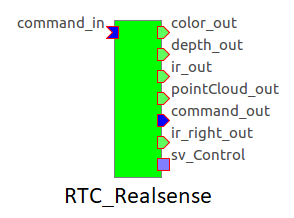
\includegraphics[width=0.4\linewidth]{fig/chp3/RealsenseDiag.png}
    \caption{Port configuration of RTC\_Realsense.}
    \label{fig:system:rtc-realsense}
\end{figure}

\paragraph{RTC\_PointCloudProcess}

RTC\_PointCloudProcessは，\ref{sec:system:software:pcl}節で述べたPCLを用いて，RTC\_Realsenseから受信した点群データを処理するRTCである．
処理の基本的な流れは以下の通りである：

\begin{enumerate}
    \item Pythonのメインスクリプトがサービスポートを通じて処理命令とパラメータをRTC\_PointCloudProcessに送信する．
    \item RTC\_PointCloudProcessがデータポートから点群を読み出す．
    \item \ref{sec:system:pointcloud:processing:pipeline}節で詳述するアルゴリズムにより点群を処理する．
    \item 処理結果をサービスポート経由でメインスクリプトに返す．
\end{enumerate}


RTC\_PointCloudProcessのポート構成を図\ref{fig:system:rtc-pointcloud-process}に，RTC全体の接続状況を図\ref{fig:system:rtc-overall-connections}に示す．

\begin{figure}[ht]
    \centering
    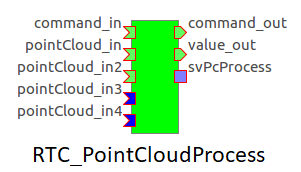
\includegraphics[width=0.4\linewidth]{fig/chp3/PointCloudProcessDiag.png}
    \caption{Port configuration of RTC\_PointCloudProcess.}
    \label{fig:system:rtc-pointcloud-process}
\end{figure}

\begin{figure}[ht]
    \centering
    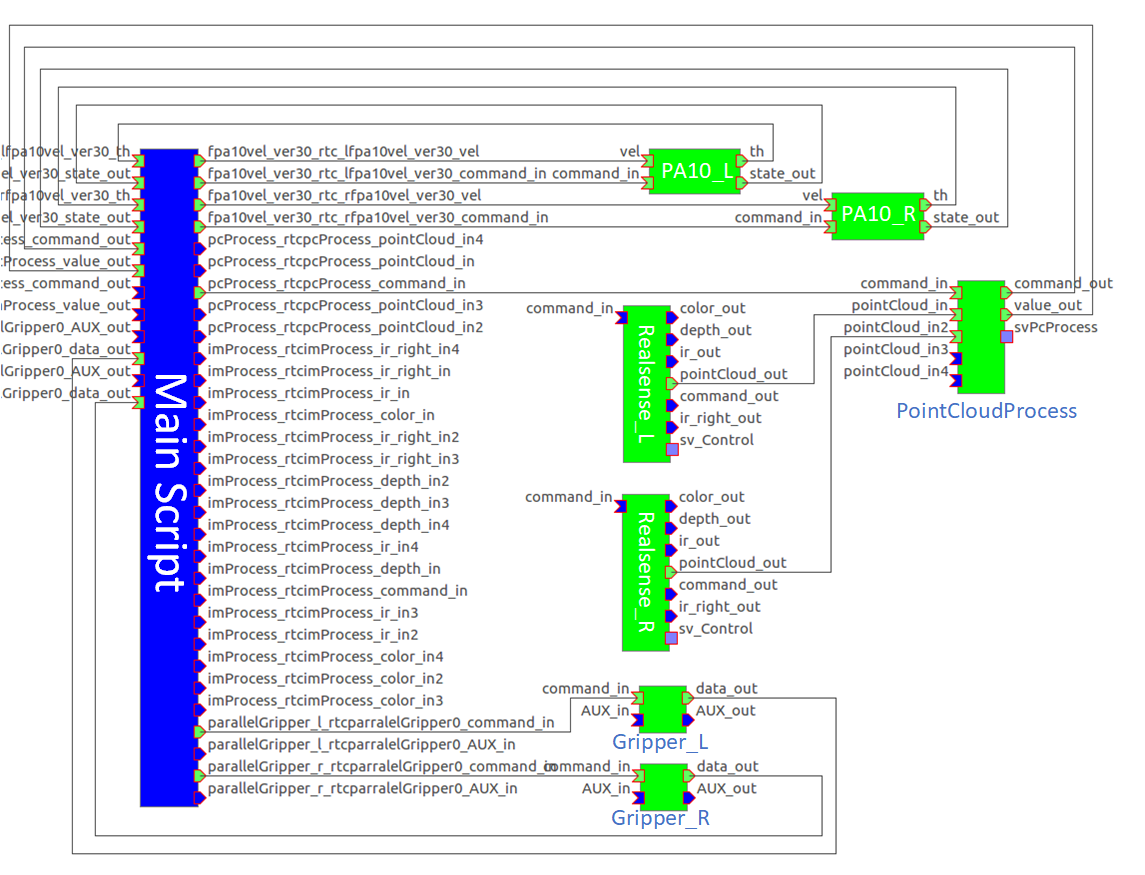
\includegraphics[width=0.9\linewidth]{fig/chp3/SystemDiag.png}
    \caption{Overall RTC connections.}
    \label{fig:system:rtc-overall-connections}
\end{figure}


\section{3D点群モデルの位置づけと全体パイプライン}
\label{sec:system:pointcloud:overview}

\subsection{本論文における点群モデルの役割}
\label{sec:system:pointcloud:role}
% TODO：RGB-Dカメラなどの深度センサにより非接触で取得可能である．这句话为什么要写？
\revise{本論文では，液体の注ぎ，食材の皮むき，および切断中の安定把持という三つの物体操作について，3次元点群モデルを共通の入力表現として用いる．}
点群モデルとは，対象物体表面の3次元座標点の集合であり，RGB-Dカメラなどの深度センサにより非接触で取得可能である．

具体的には，以下の各タスクにおいて点群モデルが中心的な役割を果たす：

\begin{enumerate}
  \item \textbf{食材の皮むき軌道生成}：皮むきタスクでは，食材表面の点群から法線ベクトルを計算し，皮むき軌道の事前生成および回転角度の算出に利用する．
  \item \textbf{容器の形状モデリング}：液体注ぎタスクでは，注ぐ容器および注ぎ先容器の内部形状を点群モデルとして取得し，容積計算することおよび液面高さから注いた量を計算するために用いる．
  \item \textbf{食材の表面形状取得}：食材把持タスクでは，食材の3次元形状を点群として取得し，把持位置探索のための幾何学的入力とする．
\end{enumerate}

これらのタスクに共通して，点群モデルは「対象物の幾何学的情報を計算機上で扱うための中間表現」として機能する．
点群表現を採用する理由は以下の通りである．
第一に，RGB-Dカメラの出力が深度画像（すなわちピクセル単位の3次元座標の集合）であり，点群表現がセンサ出力との親和性に最も優れること．
第二に，メッシュなどの表現と比較して，データ構造が単純であり，フィルタリング，ダウンサンプリング，領域分割といった処理の計算コストが低いこと．
第三に，容器の口縁検出，食材曲面追跡，把持点の探索などといった本研究が扱うタスクのいずれにおいても，物体表面の離散的なサンプリング点集合で十分な情報が得られることである．

各タスク固有の処理へ進む前に，共通する処理パイプラインを経由することで，後続のアルゴリズムへの入力品質を保証する設計となっている．

\subsection{点群取得・処理パイプラインの概要}
\label{sec:system:pointcloud:pipeline-overview}
本論文における3D点群モデル取得の共通処理パイプラインを図\ref{fig:system:pointcloud-pipeline}に示す．
パイプラインは大きく「点群取得」と「点群処理」の2段階に分けられる．

\begin{figure}[t]
  \centering
  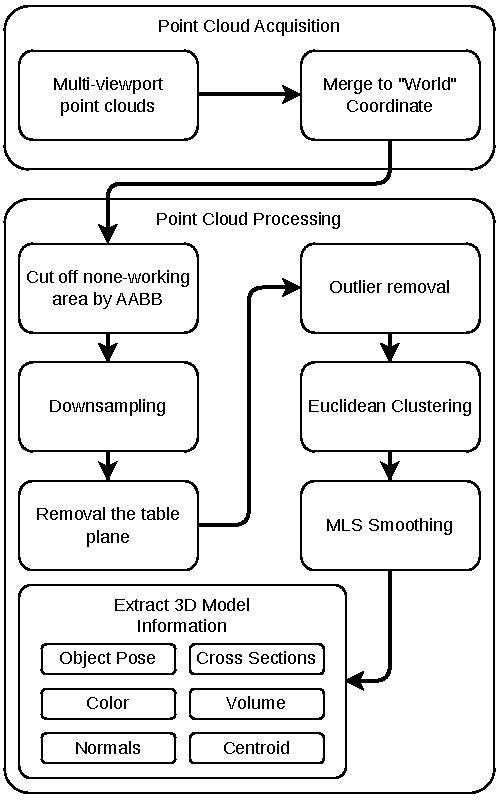
\includegraphics[width=0.6\linewidth]{fig/chp3/chp3_algo_flowchart.drawio.pdf}
  \caption{The pipeline for 3D point cloud model acquisition.}
  \label{fig:system:pointcloud-pipeline}
\end{figure}

\textbf{点群取得}では，RGB-Dカメラを用いて多視点から撮影した点群を，座標変換により合成し，対象物体の全周的な3次元形状を復元する．
この段階では，カメラキャリブレーション，座標系定義，多視点合成が主要な処理となる．

\textbf{点群処理}では，合成された点群に対して，作業領域の切り出し，ダウンサンプリング，作業台平面の除去，外れ値除去，クラスタリング，平滑化および法線ベクトル推定を順次適用し，後段のタスクに適した点群モデルを生成する．
この処理順序には必然性がある．
まず粗い空間フィルタ（作業領域切り出し）で計算負荷を低減し，次に密度均一化（ダウンサンプリング）により，この後の処理のパラメータは点群データの密度に依存させずに設定可能とする．
その上でテーブル平面除去，統計的なノイズ除去（外れ値除去），クラスタリングを経て，最後に表面の平滑化と法線推定を行う．

\section{3D点群モデルの取得}
\label{sec:system:pointcloud:acquisition}

\subsection{RGB-Dカメラによる点群取得}
\label{sec:system:pointcloud:acquisition:rgbd}
\ref{sec:system:hardware:vision-sensor}節で述べたRGB-Dカメラ（Intel RealSense D435）を用いて，対象物体の点群を撮影する．
本サブセクションでは，深度画像から3次元点群への変換メカニズムを述べる．

RealSense D435はアクティブステレオ方式により深度情報を取得し，RGB画像と深度画像を同時に出力する．
得られた深度画像とカメラ内部パラメータ（焦点距離 $f_x, f_y$，光学中心 $c_x, c_y$）から，ピンホールカメラモデルに基づく逆投影により，各ピクセルの3次元座標を計算する：

\begin{equation}
  \begin{bmatrix} X_C \\ Y_C \\ Z_C \end{bmatrix}
  = d \cdot
  \begin{bmatrix}
    \frac{1}{f_x} & 0 & -\frac{c_x}{f_x} \\
    0 & \frac{1}{f_y} & -\frac{c_y}{f_y} \\
    0 & 0 & 1
  \end{bmatrix}
  \begin{bmatrix} u \\ v \\ 1 \end{bmatrix}
  \label{eq:system:back_projection}
\end{equation}

ここで，$(u, v)$ は画像座標，$d$ は対応する深度値，$(X_C, Y_C, Z_C)$ はカメラ座標系 $\Sigma_C$ における3次元座標である．
カメラ座標系の原点はカメラの光学中心，$Z_C$ 軸は光学軸方向に設定する．

RGB-Dカメラの単一視点からの撮影では，対象物体の自己遮蔽や環境遮蔽により不可視となる領域が生じる．
このため，ロボットアームを動作させてカメラ姿勢を変更し，複数視点から点群を取得する必要がある．



\subsection{座標変換と多視点点群の合成}
\label{sec:system:pointcloud:acquisition:multi-view-fusion}
複数視点からの点群を合成する手順を以下に示す：

\begin{enumerate}
  \item ロボットアームを制御し，カメラが対象物体を取り囲むように複数の姿勢へ移動させる．
  \item 各姿勢においてRGB-Dカメラで点群を撮影し，カメラ座標系での点群 $\mathcal{P}_{C}^{(i)}$ を得る．
  \item 式(\ref{eq:system:transform_chain})に従い，各カメラ座標系の点群を世界座標系へ変換する：
  \begin{equation}
    \mathcal{P}_{W}^{(i)} = \left\{ {}^{W}\bm{T}_{H}^{(i)} \cdot {}^{H}\bm{T}_{C} \cdot \bm{p} \;|\; \bm{p} \in \mathcal{P}_{C}^{(i)} \right\}
  \end{equation}
  \item 全視点の点群を合成し，1つの点群 $\mathcal{P}_{\mathrm{all}}$ を得る：
  \begin{equation}
    \mathcal{P}_{\mathrm{all}} = \bigcup_{i=1}^{N_v} \mathcal{P}_{W}^{(i)}
  \end{equation}
  ここで，$N_v$ は視点数である．
\end{enumerate}

多視点合成により，対象物体の全周的な点群モデルが得られるが，重複領域の密度が不均一になる点や，位置姿勢誤差の蓄積による多重像が生じる点に留意する必要がある．

% \subsection{底面点群の取得}
% \label{sec:system:pointcloud:acquisition:bottom-surface}
% \paragraph{本章における位置づけ}

% 前節で述べた多視点点群合成処理により，対象物体のほぼ全周的な3次元形状が取得される．
% しかし，机上に置かれた物体を上方および側方からスキャンする構成では，底面（作業台との接触面付近）は不可視領域となる．
% 本節では，ロボットの把持機能を活用して物体を持ち上げ，底面を含む全周点群を取得する手法について述べる．

% \paragraph{卓上スキャンにおける不可視領域}

% 図\ref{fig:system:occlusion}に示すように，作業台上に静置された物体をRGB-Dカメラで多視点からスキャンしても，物体底面および作業台との接触部近傍の点群は原理的に取得不可能である．
% この不可視領域は，以下に起因する：

% \begin{enumerate}
%   \item 物体と作業台の接触による物理的遮蔽
%   \item カメラの俯角限界（アームの可動範囲制約）
%   \item 物体側面のオーバーハング形状による自己遮蔽
% \end{enumerate}

% \begin{figure}[t]
%   \centering
%   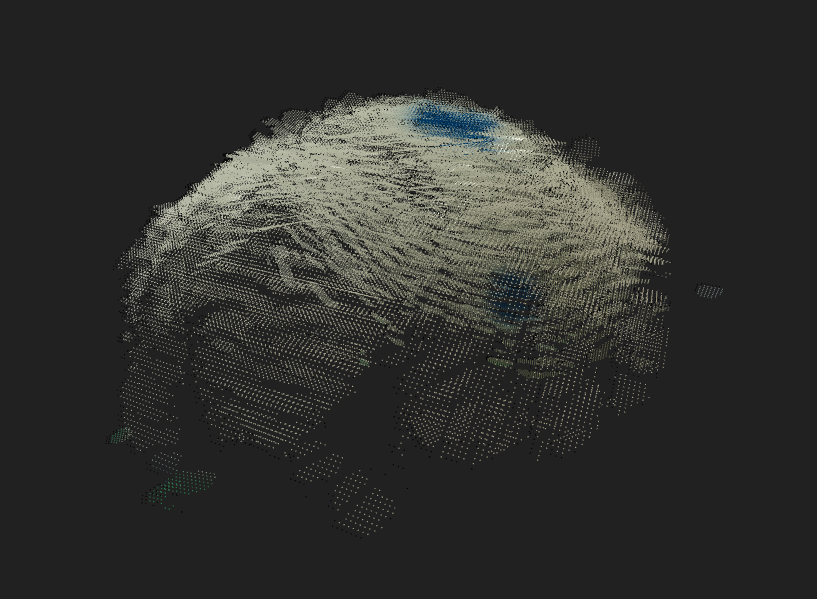
\includegraphics[width=0.70\linewidth]{fig/chp3/pointalgo_occlusion.png}
%   \caption{Invisible region in tabletop scanning.}

%     \label{fig:system:occlusion}
% \end{figure}

% % 底面情報の欠落は，特に容器の体積計算精度に重大な影響を及ぼす．
% % 例えば，深くて細い容器では底面付近の形状復元が不完全となるため，式(\ref{eq:volume_integral})の積分下限付近の誤差が累積し，全体の体積誤差が増大する．

% \paragraph{計算}

% ロボットハンドにより物体を把持して持ち上げた状態で，物体底面をカメラで撮影する．
% このとき，把持後の物体は手先座標系に対して固定されているため，撮影された底面点群は以下の座標変換により世界座標系の既存点群と合成される：

% \begin{equation}
%   \mathcal{P}_{\mathrm{bottom}}^{(W)} = \left\{ {}^{W}\bm{T}_{H}^{(g)} \cdot {}^{H}\bm{T}_{C} \cdot \bm{p} \;|\; \bm{p} \in \mathcal{P}_{\mathrm{bottom}}^{(C)} \right\}
%   \label{eq:system:bottom_transform}
% \end{equation}

% ここで，${}^{W}\bm{T}_{H}^{(g)}$ は底面撮影時のロボット手先の順運動学解，$\mathcal{P}_{\mathrm{bottom}}^{(C)}$ はカメラ座標系における底面点群である．

% 既存の点群モデル $\mathcal{P}_{\mathrm{obj}}$ と底面点群 $\mathcal{P}_{\mathrm{bottom}}^{(W)}$ の合成は，ICP（Iterative Closest Point）アルゴリズムによる精密位置合わせの後に実施する：

% \begin{equation}
%   \mathcal{P}_{\mathrm{full}} = \mathcal{P}_{\mathrm{obj}} \cup \mathcal{P}_{\mathrm{bottom}}^{(W, \mathrm{aligned})}
%   \label{eq:system:full_model}
% \end{equation}

% \paragraph{手順}

% 把持を利用した底面点群取得の手順を以下に示す：

% \begin{enumerate}
%   \item \textbf{三指把持による対象物の持ち上げ}：
%   事前に計画された把持位置に基づき，ロボットハンドの3指で対象物体を把持し，作業台から十分な高さ（約150\,mm）まで持ち上げる．
%   持ち上げ高さは，カメラの最小撮影距離と作業台の映り込み回避を考慮して決定する．

%   \item \textbf{底面点群の撮影と座標変換}：
%   持ち上げ状態で，カメラを物体の下方に向け，底面の点群を撮影する．
%   必要に応じてハンドのリストロール軸を回転させ，複数の底部視点を取得する．
%   撮影された各底面点群は，式(\ref{eq:system:bottom_transform})により世界座標系へ変換する．

%   \item \textbf{既存点群との位置合わせと合成}：
%   底面点群と既存の物体点群モデルの重複領域（側面下部）を用いてICPによる精密位置合わせを行う．
%   位置合わせ後，式(\ref{eq:system:full_model})により両者を合成し，底面を含む完全な物体モデルを生成する．
% \end{enumerate}

\subsection{底面点群の取得}
\label{sec:system:bottom_acquisition}

\ref{sec:system:pointcloud:acquisition:multi-view-fusion}節で述べた多視点合成により，対象物の上面および側面の大部分は取得できる．
しかし，対象物が作業台上に置かれている限り，作業台との接触面およびその近傍は，カメラ視線が到達しない不可視領域として残る．
この欠落は，対象物の外表面点群を全周モデルとして扱う処理に影響する．
\revise{卓上スキャンのみで得られる点群は，上面および側面のみの観測であり，底面側の点，法線，および外形の完全性が欠落する．}
そのため，食材や不定形物体の外形モデルを用いた把持候補生成，幾何学的重心の近似，および外形再構成精度の評価では，観測方向に依存した偏りが生じる可能性がある．
\begin{revisionblock}
この問題に対し，本研究では対象物を把持して作業台から持ち上げ，底面側を観測可能な状態へ能動的に変換した後，複数の提示姿勢で点群を取得する．
平面上に置かれた不規則形状物体の下面は，卓上カメラの視点数を増やすだけでは原理的に取得できない．
ロボットの把持動作を視点生成手段として利用し，持ち上げ前後の手先姿勢から点群を元の物体姿勢へ戻して統合する点は，後続タスクのための単なる前処理にとどまらず，不可視面を補完する本研究の計測上の寄与である．
\end{revisionblock}
% 本手法のポイントは，対象物を把持して提示姿勢を変化させるだけでなく，同一の把持姿勢および同一の提示姿勢列に対して，ハンドのみの点群と対象物を含む点群を対で取得する点にある．
% これにより，ロボットハンドのCADモデルを明示的に用いずに，観測点群からハンド領域を除去し，対象物表面のみを抽出できる．


% \subsubsection{底面点群取得の方針}
% \label{sec:system:bottom_acquisition_policy}

% テーブル上に置いた物体を上および側面から撮影する方法では，物体とテーブル平面が接触しているため，底面は観測できない領域として残る．
% 本研究では，この観測できない領域を補完するため，対象物をサーボハンドで把持してテーブル平面から持ち上げ，底面側をRGB-Dカメラから観測可能な状態にする．
% % TODO:少了一句核心的复原到底面位置，删除手指才是顺带的．
% ただし，持ち上げた状態で取得した点群には，対象物だけでなくサーボハンドも含まれる．
% そのため，本手法では，サーボハンドのみを撮影した点群を用いてハンド領域を除去し，得られた底面側点群をテーブル上に置かれていたときの姿勢へ復元する．

% 本節では，点群を以下の三種類に分けて扱う．
% テーブル上に置いた物体の可視部分の点群を$\mathcal{P}_{\mathrm{top}}$，対象物を持ち上げた姿勢で取得した底面側の点群を${}^{}\mathcal{P}_{\mathrm{bot1}}$，それをテーブル上の姿勢へ復元した点群を$\mathcal{P}_{\mathrm{bot2}}$と表す．

% この復元では，把持中に対象物とロボットの手先の相対姿勢が変化しないと仮定する．
% すなわち，対象物の点群は，ロボットの手先座標系$\Sigma_H$から見ると同じ位置にあるとみなす（すなわち，${}^{H1}\mathcal{P}_{\mathrm{bot1}}={}^{H2}\mathcal{P}_{\mathrm{bot2}}$）．
% この仮定に基づき，持ち上げた姿勢で得られた底面側点群を，ロボットの手先姿勢を用いてテーブル上の姿勢へ変換する．

% \subsubsection{底面点群取得の処理の流れ}
% \label{sec:system:bottom_acquisition_flow}

% \paragraph{把持の関節角度の記録}
% まず，対象物をテーブル上に置いた状態でサーボハンドを閉じ，対象物に安定接触（末端サーボのトルクが閾値以上）した時点の各サーボ関節の角度を保存する．
% 対象物なしでサーボハンドのみを撮影する場合と，対象物を把持して撮影する場合とで同じ把持の関節角度を用いることで，ハンド形状をできるだけ一致させる．
% また，このときのロボットの手先姿勢を，テーブル上の基準姿勢として記録する．
% この手先姿勢を${}^{W}\bm{T}_{H2}^{\mathrm{}}$とする．
% ここで，${}^{W}\bm{T}_{H2}^{\mathrm{}}$はテーブル上の基準姿勢における手先座標系から世界座標系への変換である．

% \paragraph{可視部分${}^{W}\mathcal{P}_{\mathrm{top}}$の取得}
% 次に，対象物をテーブル上に置いた状態で，上方および側方から撮影を行い，可視部分の点群${}^{W}\mathcal{P}_{\mathrm{top}}$を取得する．
% % この点群には，上面および側面の多くが含まれる一方で，底面およびテーブル平面との接触部近傍は含まれない．

% \paragraph{底面側点群の取得}
% 続いて，保存した把持の関節角度を用いて対象物を把持し，テーブル平面から持ち上げる．
% この状態で，RGB-Dカメラにより底面および下部側面を撮影する．
% 得られた点群は，\ref{sec:system:camera_calibration}節で述べたカメラ外部パラメータと撮影時のロボット姿勢に基づき，世界座標系へ変換される．
% この点群を${}^{W}\mathcal{P}_{\mathrm{bot1}}$とする．
% また，この撮影時の手先姿勢を${}^{W}\bm{T}_{H}^{\mathrm{lift}}$とする．

% \paragraph{ハンド領域の除去}
% 持ち上げ状態で取得した点群には，対象物表面だけでなくサーボハンド表面の点も含まれる．
% そこで，同じ把持の関節角度を対象物なしで再現し，サーボハンドのみの点群を取得する．
% 対象物を把持した点群とサーボハンドのみの点群は，同じ手先姿勢および同じ把持の関節角度で取得されるため，サーボハンド表面に対応する点はほぼ同じ空間位置に現れる．
% このため，対象物を把持した点群のうち，サーボハンドのみの点群に近い点をハンド領域として除去する．
% この処理により，サーボハンドのCADモデルを用いずに，底面側の対象物点群${}^{W}\mathcal{P}_{\mathrm{bot1}}$を抽出する．

% \paragraph{テーブル上の姿勢への復元と統合}
% ${}^{W}\mathcal{P}_{\mathrm{bot1}}$は世界座標系で表されているが，対象物は持ち上げられた姿勢にある．
% したがって，この点群をそのまま${}^{W}\mathcal{P}_{\mathrm{top}}$に加えることはできない．
% そこで，把持中に対象物と手先座標系$\Sigma_H$との相対姿勢が変化しないという仮定に基づき，${}^{W}\mathcal{P}_{\mathrm{bot1}}$をテーブル上の姿勢へ復元する．

% 持ち上げ状態で観測された底面側の点を${}^{W}\bm{p}_{\mathrm{bot1}}$，テーブル上の姿勢へ復元した点を${}^{W}\bm{p}_{\mathrm{bot2}}$とすると，両者の関係は次式で表される．

% % \begin{equation}
% %   {}^{W}\bm{p}_{\mathrm{bot2}}
% %   =
% %   {}^{W}\bm{T}_{H}^{\mathrm{table}}
% %   \left(
% %     {}^{W}\bm{T}_{H}^{\mathrm{lift}}
% %   \right)^{-1}
% %   {}^{W}\bm{p}_{\mathrm{bot1}}
% %   \label{eq:system:bottom_restore_point}
% % \end{equation}
% \begin{equation}
% \begin{aligned}
%   {}^{W}\bm{p}_{\mathrm{bot2}}
%   &=
%   {}^{W}\bm{T}_{H2}
%   \,
%   {}^{H2}\bm{p}_{\mathrm{bot2}}
%   \\
%   &=
%   {}^{W}\bm{T}_{H2}
%   \,
%   {}^{H1}\bm{p}_{\mathrm{bot1}}
%   \\
%   &=
%   {}^{W}\bm{T}_{H2}
%   \,
%   {}^{H1}\bm{T}_{W}
%   \,
%   {}^{W}\bm{p}_{\mathrm{bot1}}
% \end{aligned}
% \label{eq:system:bottom_restore_point}
% \end{equation}

% この式は，持ち上げ状態の点を一度手先座標系$\Sigma_H$へ戻し，その後，テーブル上の基準姿勢における手先姿勢へ変換することを表す．
% 式\ref{eq:system:bottom_restore_point}の1-2行の${}^{H1}\mathcal{P}_{\mathrm{bot1}}$を${}^{H2}\mathcal{P}_{\mathrm{bot2}}$に入れ替われるのは\ref{sec:system:bottom_acquisition_policy}節最後の段落の${}^{H1}\mathcal{P}_{\mathrm{bot1}}={}^{H2}\mathcal{P}_{\mathrm{bot2}}$の仮定です．

% 最後に，上方および側方から撮影して得られた可視部分${}^{W}\mathcal{P}_{\mathrm{top}}$と，テーブル上の姿勢へ復元された底面側点群${}^{W}\mathcal{P}_{\mathrm{bot2}}$を統合する．

% \begin{equation}
%   {}^{W}\mathcal{P}_{\mathrm{full}}
%   =
%   {}^{W}\mathcal{P}_{\mathrm{top}}
%   \cup
%   {}^{W}\mathcal{P}_{\mathrm{bot2}}
%   \label{eq:system:bottom_full_cloud}
% \end{equation}

% ここで得られる${}^{W}\mathcal{P}_{\mathrm{full}}$は，テーブル上に置いた状態で観測できる上面・側面点群に，持ち上げ撮影によって得られた底面および下部側面を加えた外表面点群である．
% この点群は，対象物外形の補完，法線推定，幾何学的重心の近似，および把持候補生成のために用いる．




















\subsubsection{底面点群取得の方針}
\label{sec:system:bottom_acquisition_policy}

テーブル上に置いた物体を上方および側方から撮影する方法では，物体とテーブル平面が接触しているため，底面は観測できない領域として残る．
本研究では，この観測できない領域を補完するため，対象物をサーボハンドで把持してテーブル平面から持ち上げ，底面側をRGB-Dカメラから観測可能な状態にする．
本手法の中心は，持ち上げた姿勢で得られた底面側点群を，ロボットの手先姿勢の変化に基づいて，物体がテーブル上に置かれていたときの姿勢へ復元する点にある．
ただし，持ち上げた状態で取得した点群には対象物だけでなくサーボハンドも含まれるため，復元の前にサーボハンドに由来する点を除去する．

本節では，点群を以下の三種類に分けて扱う．
テーブル上に置いた物体の可視部分の点群を${}^{W}\mathcal{P}_{\mathrm{top}}$，対象物を持ち上げた姿勢で取得した底面側の点群を${}^{W}\mathcal{P}_{\mathrm{bot1}}$，それをテーブル上の姿勢へ復元した点群を${}^{W}\mathcal{P}_{\mathrm{bot2}}$と表す．
左上の$W$は，点群が世界座標系$\Sigma_W$で記述されていることを示す．
また，持ち上げ撮影時の手先座標系を$\Sigma_{H_1}$，テーブル上の基準姿勢における手先座標系を$\Sigma_{H_2}$とする．

復元では，把持中に対象物とロボットの手先の相対姿勢が変化しないと仮定する．
したがって，同じ対象物表面点は，$\Sigma_{H_1}$から見ても$\Sigma_{H_2}$から見ても同じ手先座標値を持つとみなせる．
この関係を用いて，持ち上げ姿勢で得られた${}^{W}\mathcal{P}_{\mathrm{bot1}}$を，テーブル上の姿勢に対応する${}^{W}\mathcal{P}_{\mathrm{bot2}}$へ変換する．

\subsubsection{底面点群取得の処理の流れ}
\label{sec:system:bottom_acquisition_flow}

\paragraph{把持の関節角度と基準姿勢の記録}
まず，対象物をテーブル上に置いた状態でサーボハンドを閉じ，対象物に安定接触した時点の各サーボ関節の角度を保存する．
ここで保存する把持の関節角度は，対象物なしでサーボハンドのみを撮影する場合と，対象物を把持して撮影する場合とで，ハンド形状を一致させるために用いる．
また，このときのロボットの手先姿勢を，テーブル上の基準姿勢として記録する．
この手先姿勢を${}^{W}\bm{T}_{H_2}$とする．
ここで，${}^{W}\bm{T}_{H_2}$は，テーブル上の基準姿勢における手先座標系$\Sigma_{H_2}$から世界座標系$\Sigma_W$への変換である．

\paragraph{可視部分${}^{W}\mathcal{P}_{\mathrm{top}}$の取得}
次に，対象物をテーブル上に置いた状態で，上方および側方から撮影を行い，可視部分の点群${}^{W}\mathcal{P}_{\mathrm{top}}$を取得する．
この点群には，物体の上面および側面が含まれるが，底面およびテーブル平面との接触部近傍は含まれない．

\paragraph{底面側点群の取得}
続いて，保存した把持の関節角度を用いて対象物を把持し，テーブル平面から持ち上げる．
この状態で，RGB-Dカメラにより底面および下部側面を撮影する．
得られた点群は，\ref{sec:system:camera_calibration}節で述べたカメラ外部パラメータと撮影時のロボット姿勢に基づき，世界座標系へ変換される．
また，この撮影時の手先姿勢を${}^{W}\bm{T}_{H_1}$とする．
ここで，${}^{W}\bm{T}_{H_1}$は，持ち上げ撮影時の手先座標系$\Sigma_{H_1}$から世界座標系$\Sigma_W$への変換である．

\paragraph{ハンド領域の除去}
持ち上げ状態で取得した点群には，対象物表面だけでなくサーボハンド表面の点も含まれる．
そこで，同じ把持の関節角度を対象物なしで再現し，サーボハンドのみの点群を取得する．
対象物を把持した点群のうち，サーボハンドのみの点群に近い点をハンド領域として除去し，残った点群を持ち上げ姿勢における底面側点群${}^{W}\mathcal{P}_{\mathrm{bot1}}$とする．
この処理により，サーボハンドのCADモデルを用いずに，対象物の底面側点群を抽出できる．

\paragraph{テーブル上の姿勢への復元と統合}
${}^{W}\mathcal{P}_{\mathrm{bot1}}$は世界座標系で表されているが，対象物は持ち上げられた姿勢にある．
したがって，この点群をそのまま${}^{W}\mathcal{P}_{\mathrm{top}}$に加えることはできない．
そこで，手先姿勢${}^{W}\bm{T}_{H_1}$および${}^{W}\bm{T}_{H_2}$を用いて，${}^{W}\mathcal{P}_{\mathrm{bot1}}$をテーブル上の姿勢へ復元する．

持ち上げ状態で観測された底面側の点を${}^{W}\bm{p}_{\mathrm{bot1}}$，テーブル上の姿勢へ復元した点を${}^{W}\bm{p}_{\mathrm{bot2}}$とすると，両者の関係は次式で表される．

\begin{equation}
\begin{aligned}
  {}^{W}\bm{p}_{\mathrm{bot2}}
  &=
  {}^{W}\bm{T}_{H_2}
  \,
  {}^{H_2}\bm{p}_{\mathrm{bot2}}
  \\
  &=
  {}^{W}\bm{T}_{H_2}
  \,
  {}^{H_1}\bm{p}_{\mathrm{bot1}}
  \\
  &=
  {}^{W}\bm{T}_{H_2}
  \left(
    {}^{W}\bm{T}_{H_1}
  \right)^{-1}
  {}^{W}\bm{p}_{\mathrm{bot1}}
\end{aligned}
\label{eq:system:bottom_restore_point}
\end{equation}

式\eqref{eq:system:bottom_restore_point}の1行目は，復元後の点${}^{W}\bm{p}_{\mathrm{bot2}}$を，テーブル上の基準姿勢における手先座標${}^{H_2}\bm{p}_{\mathrm{bot2}}$から世界座標系へ変換することを表す．
2行目では，把持中に対象物と手先の相対姿勢が変化しないという仮定を用い，${}^{H_2}\bm{p}_{\mathrm{bot2}}$を持ち上げ撮影時の手先座標${}^{H_1}\bm{p}_{\mathrm{bot1}}$に置き換えている．
3行目では，持ち上げ状態で世界座標系に表されている点${}^{W}\bm{p}_{\mathrm{bot1}}$を，$\left({}^{W}\bm{T}_{H_1}\right)^{-1}$により手先座標系$\Sigma_{H_1}$へ変換している．
したがって，式\eqref{eq:system:bottom_restore_point}は，持ち上げ状態の底面側点群を一度手先座標系へ戻し，その後，テーブル上の基準姿勢における手先姿勢へ写す変換である．

点群全体に式\eqref{eq:system:bottom_restore_point}を適用することで，テーブル上の姿勢へ復元された底面側点群${}^{W}\mathcal{P}_{\mathrm{bot2}}$を得る．
最後に，上方および側方から撮影して得られた可視部分${}^{W}\mathcal{P}_{\mathrm{top}}$と，復元された底面側点群${}^{W}\mathcal{P}_{\mathrm{bot2}}$を統合する．

\begin{equation}
  {}^{W}\mathcal{P}_{\mathrm{full}}
  =
  {}^{W}\mathcal{P}_{\mathrm{top}}
  \cup
  {}^{W}\mathcal{P}_{\mathrm{bot2}}
  \label{eq:system:bottom_full_cloud}
\end{equation}

ここで得られる${}^{W}\mathcal{P}_{\mathrm{full}}$は，テーブル上に置いた状態で観測できる上面・側面点群に，持ち上げ撮影によって得られた底面および下部側面を加えた外表面点群である．
この点群は，対象物外形の補完，法線推定，幾何学的重心の近似，および把持候補生成のために用いる．








































\section{3D点群モデルの処理}
\label{sec:system:pointcloud:processing}

\subsection{処理パイプライン}
\label{sec:system:pointcloud:processing:pipeline}

合成後の点群 $\mathcal{P}_{\mathrm{all}}$ には，対象物体以外の点（作業台，背景，センサノイズなど）が含まれるため，以下の処理パイプラインを適用して対象物体の点群モデルを抽出する．
% 本処理は，表\ref{tab:system:configuration-diff}に示したいずれのアーキテクチャにおいても同一のアルゴリズムを用いて実装した（PCL\cite{PCL}，Open3D，または自作PCL-Pythonラッパー経由）．

\paragraph{作業領域の切り出し}

まず，ロボットの作業範囲外の不要な点を除去するため，世界座標系における3次元矩形領域（Axis-Aligned Bounding Box; AABB）を指定し，領域外の点をフィルタリングする．
具体的には，作業台上面を基準とした $x, y, z$ 各軸方向の範囲 $[x_{\min}, x_{\max}] \times [y_{\min}, y_{\max}] \times [z_{\min}, z_{\max}]$ を経験的に設定し，Pass-Throughフィルタを適用する．

\begin{equation}
  \mathcal{P}_{\mathrm{roi}} = \left\{ \bm{p} \in \mathcal{P}_{\mathrm{all}} \;|\; \bm{p} \in [x_{\min}, x_{\max}] \times [y_{\min}, y_{\max}] \times [z_{\min}, z_{\max}] \right\}
  \label{eq:system:roi}
\end{equation}

これにより，後段処理の計算負荷が低減されるとともに，背景領域の誤検出が抑制される．

\paragraph{ダウンサンプリング}

多視点合成後の点群は高密度であり，後段の処理を効率化するため，Voxel Gridフィルタを用いてダウンサンプリングを行う．

Voxel Gridフィルタでは，3次元空間を一辺 $l_v$ のボクセル格子に分割し，各ボクセル内の点群をその重心位置で代表する：

\begin{equation}
  \mathcal{P}_{\mathrm{ds}} = \left\{ \frac{1}{|\mathcal{V}_k|} \sum_{\bm{p} \in \mathcal{V}_k} \bm{p} \;|\; \mathcal{V}_k \neq \emptyset \right\}
\end{equation}

ここで，$\mathcal{V}_k$ は $k$ 番目のボクセルに含まれる点の集合，$|\mathcal{V}_k|$ はその点数を表す．
本論文では，ボクセルサイズ $l_v = 1.0$\,mm を基本値とし，タスクに応じて調整する．
ダウンサンプリングにより，点群の密度が均一化され，かつ計算量が大幅に削減される．

\paragraph{作業台平面の除去}

作業領域内には，対象物体に加えて作業台平面が含まれている．
作業台平面は Random Sample Consensus（RANSAC）\cite{PCL-RANSAC} を用いて検出・除去する．

RANSACによる平面検出では，以下の処理を反復する：
% TODO: 3点？PCL是这样么
\begin{enumerate}
  \item 点群から3点をランダムに選択し，それらが定義する平面モデル $ax + by + cz + d = 0$ を生成する．
  \item 全点に対して，平面モデルからの距離が閾値 $\epsilon_p$ 以内の点をインライアとして集計する．
  \item 十分な反復回数の後，最多のインライア数を得た平面モデルを採用する．
\end{enumerate}

採用された平面モデルに対するインライア点を点群から除去することで，作業台平面を除外する：

\begin{equation}
  \mathcal{P}_{\mathrm{noplanar}} = \mathcal{P}_{\mathrm{ds}} \setminus \left\{ \bm{p} \in \mathcal{P}_{\mathrm{ds}} \;|\; \mathrm{dist}(\bm{p}, \Pi) \leq \epsilon_p \right\}
  \label{eq:system:plane_removal}
\end{equation}

ここで，$\Pi$ は検出された平面，$\mathrm{dist}(\bm{p}, \Pi)$ は点 $\bm{p}$ と平面 $\Pi$ の直交距離である．
本論文では $\epsilon_p = 2.0$\,mm を用いた．

\paragraph{外れ値除去}

センサノイズや多重像に起因する疎な外れ値点を除去するため，Statistical Outlier Removalフィルタを適用する．
本フィルタでは，各点について $k$ 近傍点までの平均距離 $\bar{d}_i$ を計算し，全点の平均距離分布に基づいて外れ値を判定する：

\begin{equation}
  \mathcal{P}_{\mathrm{filtered}} = \left\{ \bm{p}_i \in \mathcal{P}_{\mathrm{noplanar}} \;|\; \bar{d}_i \leq \mu_d + \alpha \sigma_d \right\}
\end{equation}

ここで，$\mu_d$ は全点の近傍平均距離の平均，$\sigma_d$ は標準偏差，$\alpha$ は許容度パラメータである．
本研究では $k = 50$，$\alpha = 1.0$ を標準的に用いる．

また，PCLに実装されているRadius Outlier Removal\cite{PCL-method}も併用し，半径 $r_r$ 内に存在する近傍点数が閾値 $n_{\min}$ 未満の点を孤立点として除去する．

\paragraph{クラスタリングによる対象物抽出}

平面除去および外れ値除去後の点群には，対象物体に加えて作業台上の他の物体や残留ノイズが含まれる可能性がある．
そこで，Euclidean Clustering\cite{PCL-method}を適用し，空間的に連続する点群を個別のクラスタに分割する．

Euclidean Clusteringでは，点間のユークリッド距離が閾値 $d_{\mathrm{th}}$ 未満の場合に同一クラスタとみなす：

\begin{equation}
  \mathrm{cluster}(\bm{p}_i, \bm{p}_j) = \begin{cases}
    \text{同じクラスタ} & \text{if } \|\bm{p}_i - \bm{p}_j\| \leq d_{\mathrm{th}} \\
    \text{異なるクラスタ} & \text{otherwise}
  \end{cases}
\end{equation}

各クラスタに対して，点数 $N_{\mathrm{cluster}}$ および重心位置の評価により対象物体を同定する．
具体的には，閾値 $N_{\min}$ 以上の点数を有し，かつ重心が作業領域内の適切な位置にあるクラスタを対象物体の点群 $\mathcal{P}_{\mathrm{obj}}$ として選択する．

\paragraph{平滑化と法線ベクトル推定}

クラスタリングにより抽出された対象物体の点群 $\mathcal{P}_{\mathrm{obj}}$ に対し，Moving Least Squares（MLS）法\cite{PCL-MLS}による平滑化と法線ベクトル推定を同時に適用する．

MLS法では，各点 $\bm{p}_i$ の近傍点群に対して局所的な多項式曲面をフィッティングし，再サンプリングすることで平滑化された点群 $\mathcal{P}_{\mathrm{smooth}}$ を得る．
同時に，フィッティングされた局所曲面の法線方向として，各点の法線ベクトル $\bm{n}_i$ が計算される：

\begin{equation}
  \bm{n}_i = \frac{\partial \mathcal{S}}{\partial x} \times \frac{\partial \mathcal{S}}{\partial y} \Big|_{\bm{p}_i}
\end{equation}

ここで，$\mathcal{S}$ は局所近似曲面である．
法線ベクトルは，後段のタスク（把持位置探索，皮むき軌道生成，表面領域分割など）において必須の幾何学情報となる．

なお，MLS法の局所近似半径 $r_{\mathrm{mls}}$ は，点群密度に依存するパラメータであり，本研究では経験的に $r_{\mathrm{mls}} = 3.0$\,mm を用いる．

\subsection{点群処理パラメータ}
\label{sec:system:pointcloud:processing:parameters}
表\ref{tab:system:pointcloud-parameters}に，本章で用いる標準的な点群処理パラメータをまとめる．
これらの値は，使用するRGB-Dカメラの特性，対象物体のサイズ，および作業環境に応じて調整される．

\begin{table}[t]
  \centering
  \caption{Standard parameters for point cloud processing.}
  \label{tab:system:pointcloud-parameters}
  \begin{tabular}{lcl}
    \toprule
    \textbf{Processing step} & \textbf{Parameter} & \textbf{Standard value} \\
    \midrule
    Voxel Grid downsampling & Voxel size $l_v$ & 1.0\,mm \\
    RANSAC plane removal & Distance threshold $\epsilon_p$ & 2.0\,mm \\
    Statistical Outlier Removal & Number of neighbors $k$ & 50 \\
    Statistical Outlier Removal & Tolerance $\alpha$ & 1.0 \\
    Radius Outlier Removal & Search radius $r_r$ & 5.0\,mm \\
    Radius Outlier Removal & Minimum number of neighbors $n_{\min}$ & 10 \\
    Euclidean Clustering & Cluster distance threshold $d_{\mathrm{th}}$ & 3.0\,mm \\
    Euclidean Clustering & Minimum cluster size $N_{\min}$ & 500 \\
    MLS smoothing & Local approximation radius $r_{\mathrm{mls}}$ & 3.0\,mm \\
    \bottomrule
  \end{tabular}
\end{table}

\subsection{点群モデルから得られる基礎情報}
\label{sec:system:pointcloud:basic-information}
前処理を経て得られた点群モデル $\mathcal{P}_{\mathrm{obj}}$ から，後段のタスクを遂行するために以下の基礎情報が抽出される．

\paragraph{位置姿勢と範囲}

点群モデルのAABBや主成分を計算することにより，世界座標系における物体の位置姿勢や範囲を取得する．この情報は，ロボットアームの到達可能性判定，衝突回避，およびカメラの再撮影時の視点計画に利用される．

\paragraph{色情報}

RGB-Dカメラからは各点の3次元座標に加えて色情報（RGB値）が取得される．
色情報は主に特定色の抽出による対象領域を識別するために用いる．

\paragraph{法線ベクトル}

MLS平滑化により推定された法線ベクトル $\{ \bm{n}_i \}$ は，以下のタスクにおいて中心的役割を果たす：

\begin{enumerate}
  \item 把持位置の力学的評価（力の釣り合い解析の幾何学的入力）
  \item 物体表面の曲率評価
\end{enumerate}

% TODO：把第五章的断面面积的计算拿到这里

\paragraph{断面と体積計算}

物体の幾何学的特性を定量化するため，点群モデルから断面情報を抽出する．
容器モデルの場合，以下の手順で体積計算が可能である：

\begin{enumerate}
  \item 点群モデルを $z$ 軸方向に一定間隔 $\Delta h$（本論文では $\Delta h = 1$\,mm）でスライスする．
  \item 各スライス高さ $h_k$ において，スライス平面から閾値以内の点群を当該断面の点集合とする．
  \item 断面点群をスライス面に投影し，投影点群の凸包を Quickhull アルゴリズム\cite{PCL-Convex}により計算する．
  \item 凸包の面積 $A(h_k)$ を断面積として算出する．
  \item 全スライスの断面積を高さ方向に積分することで，任意の液面高さ $H$ までの体積 $V(H)$ を求める：
  \begin{equation}
    V(H) = \int_{0}^{H} A(h)\, dh \approx \sum_{k:\,h_k \leq H} A(h_k) \cdot \Delta h
    \label{eq:system:volume_integral}
  \end{equation}
\end{enumerate}

\revise{この断面積分法により，本研究で扱う開口容器について，個々の容器形状から体積を計算できる（図\ref{fig:system:cross-section}）．ただし，凹部や内部遮蔽によって内面点群が欠落する容器では近似誤差が生じる．}

\begin{figure}[t]
  \centering
  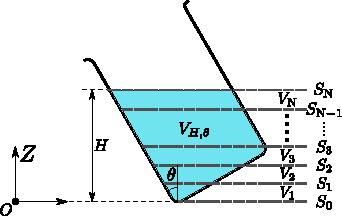
\includegraphics[width=0.75\linewidth]{fig/chp_pouring/ParametersV4.pdf}
  \caption{Conceptual diagram of point-cloud slicing and cross-sectional area calculation.}
  \label{fig:system:cross-section}
\end{figure}

\paragraph{重心}

物体の幾何学的重心 $\bm{g}$ は，点群の全点の座標平均として近似計算される：

\begin{equation}
  \bm{g} = \frac{1}{|\mathcal{P}_{\mathrm{obj}}|} \sum_{\bm{p} \in \mathcal{P}_{\mathrm{obj}}} \bm{p}
  \label{eq:system:centroid}
\end{equation}

重心位置は，把持の力学的安定性評価における重要な入力であり，特に食材把持タスクでは，食品の密度が比較的均一であるとの仮定の下，幾何学的重心を質量中心の近似値として使用する．

\paragraph{表面領域と指先位置候補}

点群モデルから，物体表面の各点を指先把持位置の候補として利用する．
具体的には，$\mathcal{P}_{\mathrm{obj}}$ の各点 $\bm{p}_i$ を指先位置候補とし，対応する法線ベクトル $\bm{n}_i$ を指先の接近方向として扱う．
これにより，多数の把持候補（最大で $K = |\mathcal{P}_{\mathrm{obj}}|$ 個）が生成される．
計算効率の観点から，事前に点群をダウンサンプリングして候補点数を制限する（例：実験では約150〜200点に制限）．

\paragraph{後続章における利用}

上記の基礎情報は，後続する各章において以下のように利用される：

\begin{enumerate}
  \item \textbf{第4章-皮むき作業}：物体表面の法線ベクトルに基づく皮むき軌道の事前生成，法線角度変化に基づく軌道セグメント化，および皮むきエッジの色情報抽出．
  \item \textbf{第5章-液体を注ぐ作業}：容器の断面積データを用いた注いだ体積計算，および液面検出のためのAABBによる領域制限．
  \item \textbf{第6章-切断時の安定把持}：表面点群を把持の探索空間とし，法線ベクトルと重心位置を用いた把持のスコア計算．
\end{enumerate}

% ============================================================
% TODO：通过程序生成


\section{3D点群モデル取得の精度評価実験}
\label{sec:system:pointcloud:evaluation}

本節では，前節までに述べた多視点点群取得，座標変換，点群処理，および基礎幾何情報抽出の精度を，実験により評価する．
本論文で用いる3D点群モデルは，後続章において皮むき軌道生成，容器容積計算，および把持点探索の入力となる．
したがって，評価では単に点群が見た目として対象物を再現できているかではなく，タスクで利用される幾何量がどの程度安定に得られるかを確認する必要がある．
この目的のため，本節では以下の三種類の実験を行った．
第一に，球および円柱という幾何学的形状が既知の標準物体を撮影し，プリミティブフィッティングにより得られる半径，軸方向，および位置の誤差を評価した．
第二に，3Dプリンタで作製した形状の異なる5種類の容器を撮影し，容積計算精度およびCADモデルに対する表面形状誤差を評価した．
第三に，卓上観測では欠落しやすい底面側の点群を把持・持ち上げによって補完する手法について，CADモデルとの距離誤差により評価した．

\subsection{評価指標}
\label{sec:system:pointcloud:evaluation:metrics}

本節の評価では，対象物と実験目的に応じて，プリミティブパラメータ誤差，点群から参照モデルへの距離誤差，および容積誤差を用いる．

\paragraph{プリミティブパラメータ誤差}

球および円柱のように幾何学的モデルが明確な標準物体では，取得点群に対して球または円柱をフィッティングし，得られたパラメータを参照値と比較する．
球体では半径$r$および中心位置$\bm{c}$を評価し，円柱では半径$r$，軸方向$\bm{v}$，および上面中心位置$\bm{c}_{\mathrm{top}}$を評価する．
推定値を$\hat{\cdot}$，参照値を下付き$\mathrm{GT}$で表すと，半径誤差，中心位置誤差，および軸方向誤差は次式で表される．

\begin{equation}
  e_r = \hat{r}-r_{\mathrm{GT}}, \quad
  \bm{e}_{c} = \hat{\bm{c}}-\bm{c}_{\mathrm{GT}}, \quad
  \bm{e}_{v} = \hat{\bm{v}}-\bm{v}_{\mathrm{GT}}.
  \label{eq:system:primitive_error}
\end{equation}

円柱軸の向きについては，ベクトル成分の誤差に加え，必要に応じて以下の角度誤差としても評価できる．

\begin{equation}
  e_{\theta}=\cos^{-1}\left(\left|\hat{\bm{v}}\cdot\bm{v}_{\mathrm{GT}}\right|\right).
  \label{eq:system:axis_angle_error}
\end{equation}

ここで絶対値を用いるのは，円柱軸の正負方向が幾何学的には同一の軸を表すためである．

\paragraph{点群--モデル間距離誤差}

3Dプリンタ製物体のように自由曲面を含む対象では，CADモデルまたは高精度に取得した参照モデルを真値形状として用いる．
まず，取得点群$P=\{\bm{p}_i\}_{i=1}^{N}$を参照モデル$M$にICPで位置合わせし，変換後の各点から参照モデル表面までの最短距離を計算する．

\begin{equation}
  d_i=\min_{\bm{q}\in M}\left\|\bm{T}_{\mathrm{ICP}}\bm{p}_i-\bm{q}\right\|.
  \label{eq:system:point_to_model_distance}
\end{equation}

この距離集合$\{d_i\}$に対して，平均値，分散，標準偏差，およびRMSEを以下のように定義する．

\begin{align}
  \bar{d} &= \frac{1}{N}\sum_{i=1}^{N}d_i, \\
  \sigma_d^2 &= \frac{1}{N}\sum_{i=1}^{N}(d_i-\bar{d})^2, \\
  \mathrm{RMSE} &= \sqrt{\frac{1}{N}\sum_{i=1}^{N}d_i^2}.
  \label{eq:system:distance_statistics}
\end{align}

実験結果の表では，分散そのものではなく，解釈しやすい標準偏差$\sigma_d$を併記する．

\paragraph{容積誤差}

容器形状の評価では，式(\ref{eq:system:volume_integral})により点群モデルから計算した容積$V_{\mathrm{estimated}}$と，水充填法により得た実測容積$V_{\mathrm{GT}}$を比較する．
絶対誤差および相対誤差を次式で定義する．

\begin{equation}
  e_{\mathrm{vol}} = V_{\mathrm{estimated}}-V_{\mathrm{GT}},
  \label{eq:system:vol_error}
\end{equation}

\begin{equation}
  e_{\mathrm{vol,rel}} = \frac{|V_{\mathrm{estimated}}-V_{\mathrm{GT}}|}{V_{\mathrm{GT}}}\times100\;[\%].
  \label{eq:system:vol_error_rel}
\end{equation}

符号付き誤差$e_{\mathrm{vol}}$は，推定値が真値に対して過大であるか過小であるかを考察するために用い，相対誤差は容器サイズが異なる場合の比較に用いる．

\subsection{標準物体の撮影実験}
\label{sec:system:pointcloud:evaluation:standard-objects}

\paragraph{実験目的と参照値}

まず，提案した点群取得・処理パイプラインの基本的な幾何精度を確認するため，形状が単純でパラメータ化しやすい標準物体を撮影した．
対象物は，3Dプリンタで作製した円柱および球体である．
直接測定による真値として，球体の直径は57.25\,mm，円柱の高さは52.5\,mm，直径は45.0\,mmであった．
さらに，ロボット手先に針を固定し，工具座標系を針先端に一致させた後，針先端を対象物表面に接触させて接触時の工具座標系姿勢を記録した．
この接触点群を用いて標準物体をフィッティングし，カメラ計測値を比較するための参照パラメータを得た．
円柱については，参照半径は22.133\,mm，軸方向は$[-0.001817, -0.004072, 0.999990]^{\mathrm{T}}$，上面中心は$[0.328219, 0.000324, 0.173146]^{\mathrm{T}}$\,mであった．
球体については，参照中心は$[0.334752, 0.003555, 0.149030]^{\mathrm{T}}$\,m，参照半径は28.147\,mmであった．

\paragraph{撮影条件と処理方法}

RGB-Dカメラと対象物との距離を150，170，190，210，250\,mmの5条件に設定し，各距離で5回ずつ撮影を行った．
撮影姿勢は，対象物の前後左右方向から内部または側面が観測できるように，10--60$^{\circ}$の範囲で斜め方向の視点を設定した．
取得した各視点点群は世界座標系へ変換した後に統合し，第\ref{sec:system:pointcloud:processing}節で述べた共通処理パイプラインを適用した．
球体については処理後の点群に球フィッティングを行い，中心および半径を推定した．
円柱については，共通処理に加えてRANSACにより上面と円柱側面を分割し，側面点群から半径および軸方向を，上面点群から上面中心位置を推定した．

\paragraph{結果}

表\ref{tab:system:standard-cylinder}に，円柱標準物体に対する距離別のフィッティング誤差を示す．
表中の半径誤差および上面中心誤差はmm単位で示し，軸方向誤差は単位ベクトルの各成分の差で示す．

\begin{table}[!t]
  \centering
  \caption{Fitting errors of the cylindrical standard object at different camera distances.}
  \label{tab:system:standard-cylinder}
  \scriptsize
  \resizebox{0.85\textwidth}{!}{%
  \begin{tabular}{llrrrrrrr}
    \toprule
    \textbf{Dist. [mm]} & \textbf{Stat.} & \textbf{Radius err. [mm]} & \multicolumn{3}{c}{\textbf{Axis direction err. [-]}} & \multicolumn{3}{c}{\textbf{Top-center err. [mm]}} \\
    \cmidrule(lr){4-6}\cmidrule(lr){7-9}
     & & & \textbf{X} & \textbf{Y} & \textbf{Z} & \textbf{X} & \textbf{Y} & \textbf{Z} \\
    \midrule
    250 & Avg. & -0.552 & 0.001787 & -0.006661 & 0.000000 & -0.881 & 0.112 & -0.001 \\
        & Std. &  0.170 & 0.000856 &  0.000785 & 0.000004 &  0.149 & 0.116 &  0.001 \\
    210 & Avg. & -0.882 & 0.004268 & -0.002733 & 0.000010 & -1.542 & 0.077 & -0.002 \\
        & Std. &  0.156 & 0.000392 &  0.001104 & 0.000002 &  0.191 & 0.058 &  0.000 \\
    190 & Avg. & -0.704 & 0.003425 & -0.005729 & 0.000005 & -0.985 & -0.069 & 1.682 \\
        & Std. &  0.149 & 0.000665 &  0.000508 & 0.000004 &  0.197 &  0.094 & 0.202 \\
    170 & Avg. & -0.660 & 0.003636 & -0.010245 & 0.000024 & -1.354 & -0.066 & 1.411 \\
        & Std. &  0.146 & 0.000453 &  0.000551 & 0.000004 &  0.249 &  0.202 & 0.802 \\
    150 & Avg. & -0.785 & 0.012453 & -0.010729 & 0.000114 & -1.267 & 0.046 & -0.002 \\
        & Std. &  0.098 & 0.000784 &  0.000285 & 0.000012 &  0.179 & 0.059 &  0.000 \\
    \midrule
    All & Avg. & -0.716 & 0.005114 & -0.007220 & 0.000031 & -1.206 & 0.020 & 0.617 \\
        & Std. &  0.175 & 0.003884 &  0.003100 & 0.000044 &  0.305 & 0.132 & 0.849 \\
    \bottomrule
  \end{tabular}%
  }
\end{table}

\paragraph{考察}

円柱半径の誤差は，すべての距離で負の値となった．
全条件平均では$-0.716$\,mmであり，標準偏差は0.175\,mmであった．
これは，取得点群から推定される円柱側面が参照半径よりもわずかに内側に寄る傾向を示している．
主な要因として，RGB-Dカメラの深度値の系統誤差，MLS平滑化による外周部の丸め込み，およびRANSACによる円柱面抽出時に外周付近の点が外れ値として除去されたことが考えられる．
一方で，各距離における半径誤差の標準偏差は0.10--0.17\,mm程度に収まっており，同一条件内での再現性は高かった．

軸方向については，$z$成分の誤差がほぼ0であり，推定された円柱軸は参照軸と同様に鉛直方向をよく保持していた．
$x$および$y$成分の誤差から近似した角度誤差は，全条件平均で約0.5$^{\circ}$であり，円柱軸の推定は十分安定であった．
ただし，150\,mm条件では$x$成分および$y$成分の誤差が他の距離より大きく，近距離撮影では深度画像の局所的な歪みや視野端での欠損が軸推定に影響しやすいことが分かる．
この結果から，本システムで標準物体や容器を撮影する場合，150\,mmのような近距離よりも，190--250\,mm程度の距離の方が安定した形状推定を行いやすいと考えられる．

上面中心位置については，$x$方向に平均$-1.206$\,mmの系統的なずれが見られた．
一方，$y$方向の平均誤差は0.020\,mmと小さく，左右方向の位置合わせは良好であった．
$z$方向では190\,mmおよび170\,mm条件で1--2\,mm程度の正の誤差が生じたが，他の距離ではほぼ0に近かった．
このことから，上面中心の位置誤差はランダムノイズだけでなく，カメラ外部パラメータ，ロボット姿勢，および上面分割の安定性に由来する成分を含むと考えられる．
後続タスクでは，数mm程度の位置誤差は力覚フィードバックや再観測により補償可能であるが，容器の縁や注ぎ口のような局所特徴を利用する場合には，撮影距離と視点配置を適切に選ぶ必要がある．

球体については，中心および半径のみを評価対象とした．
球は円柱と異なり軸方向や上面中心を持たず，RANSACによる上面・側面分割を必要としないため，処理手順は比較的単純である．
その一方で，球面の周辺部ではカメラ視線と表面法線のなす角が大きくなり，深度欠損や外れ値が生じやすい．
したがって，球体実験は曲率を有する表面の取得安定性を確認する役割を持ち，多視点合成および外れ値除去が曲面物体のモデル化に有効であることを確認するための基礎評価として位置づけられる．

\subsection{3Dプリンタ製物体の撮影実験}
\label{sec:system:pointcloud:evaluation:3d-printed-object}

\paragraph{実験目的と対象物}

\begin{figure}[!t]
    \centering
    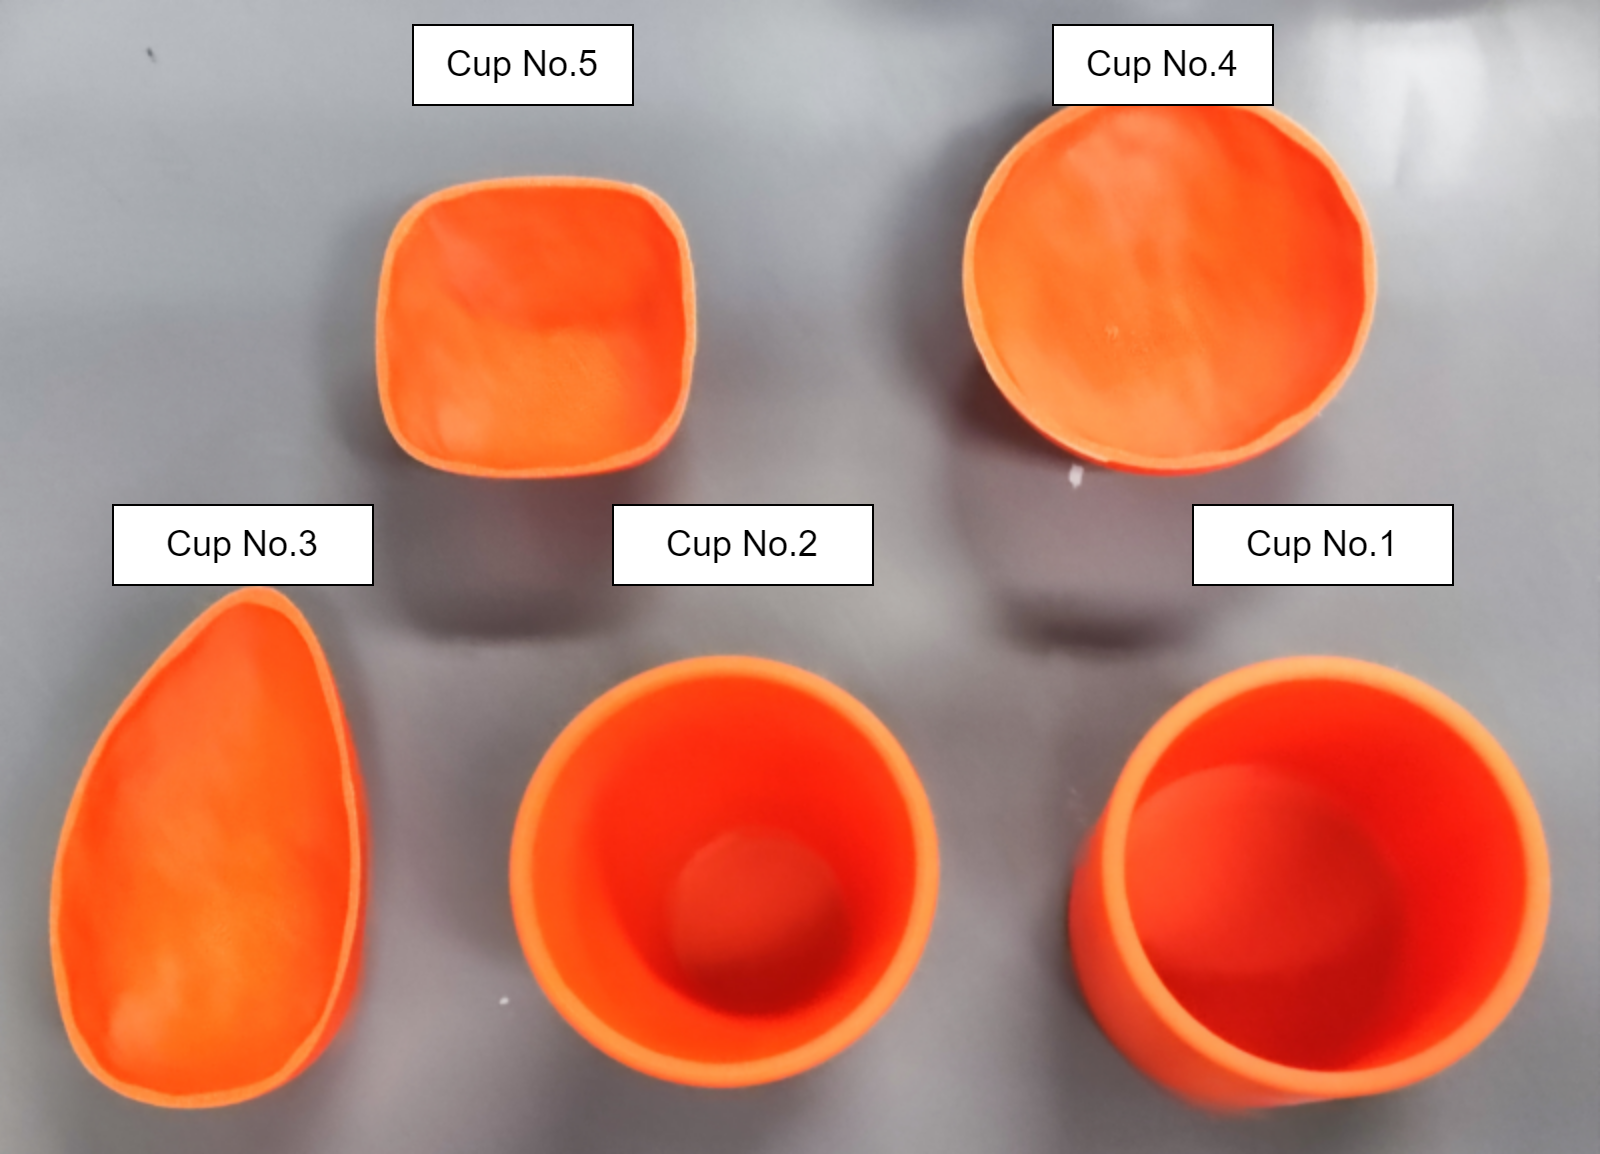
\includegraphics[width=0.7\linewidth]{fig/chp3/chp3_cups.drawio.png}
    \caption{The 3D-Printed cups used in experiment section \ref{sec:system:pointcloud:evaluation:3d-printed-object}.}
    \label{fig:system:pointcloud:evaluation:3d-printed-object}
\end{figure}

次に，標準物体よりも複雑な形状をもつ対象に対して，提案パイプラインがタスクに必要な幾何情報を抽出できるかを評価した．
対象物は，図\ref{fig:system:pointcloud:evaluation:3d-printed-object}で示した，3Dプリンタで作製した5種類の容器であり，それぞれCup 1-5と呼ぶ．
これらは開口部形状，側面曲率，底面形状，および傾斜部の有無が異なるため，容器モデル取得における典型的な形状差を含んでいる．
評価は，容積計算精度と表面形状誤差の二つの観点から行った．

\paragraph{容積計算の評価}

容積の真値は，容器に水を満たし，液面を容器上端と一致させた状態で水の重量を測定し，水の密度を用いて体積へ換算することで得た．
各容器について6回の測定を行い，その平均値を真値$V_{\mathrm{GT}}$とした．
カメラ計測値は，第\ref{sec:system:pointcloud:basic-information}節で述べた$z$方向スライスに基づく断面積分により計算した．
各スライスでは，断面点群を平面に投影し，Convex Hullの面積を断面積として求めた後，隣接スライス間の体積を台形近似で積算した．

表\ref{tab:system:container-volume}に容積計算結果を示す．
表中の設計容積は参考値であり，誤差計算には水重量測定の平均値を真値として用いた．

\begin{table}[t]
  \centering
  \caption{Volume estimation results for 3D-printed containers.}
  \label{tab:system:container-volume}
  \small
  \begin{tabular}{lrrrrr}
    \toprule
    \textbf{Object} & \textbf{Design} & \textbf{GT} & \textbf{Estimated} & \textbf{Error} & \textbf{Rel. err.} \\
     & \textbf{[$\mathrm{cm}^3$]} & \textbf{[$\mathrm{cm}^3$]} & \textbf{[$\mathrm{cm}^3$]} & \textbf{[$\mathrm{cm}^3$]} & \textbf{[\%]} \\
    \midrule
    Cup 1 & 575.48 & $569.92\pm0.97$ & 574.10 &  4.18 & 0.73 \\
    Cup 2   & 366.13 & $362.00\pm0.55$ & 374.48 & 12.48 & 3.45 \\
    Cup 3 & 194.70 & $193.38\pm0.56$ & 184.40 & -8.98 & 4.65 \\
    Cup 4 & 221.05 & $218.92\pm0.39$ & 217.88 & -1.04 & 0.47 \\
    Cup 5 & 140.83 & $141.63\pm0.70$ & 138.45 & -3.18 & 2.25 \\
    \bottomrule
  \end{tabular}
\end{table}

5種類の容器に対する平均絶対誤差は5.97\,$\mathrm{cm}^3$，平均相対誤差は2.31\%であった．
Cup 1およびCup 4では相対誤差が1\%未満であり，提案した点群取得と断面積分により，単純な円筒形状だけでなく曲面を含む容器でも高い精度で容積を推定できることが分かった．
一方，Cup 2では推定値が真値より12.48\,$\mathrm{cm}^3$大きく，Cup 3では8.98\,$\mathrm{cm}^3$小さかった．
この差は，断面積をConvex Hullで近似することによる影響と，容器内部の点群密度の偏りによる影響が大きいと考えられる．
特に，凹部やくびれを含む断面ではConvex Hullが実際の内側形状より広い領域を囲むため，体積が過大評価される可能性がある．
反対に，深い容器や角部を持つ容器では，内壁の一部が視線方向に対して隠れ，断面点群が不足することで断面積が過小評価される場合がある．
Cup 5のように開口部や側面に傾斜を含む容器では，スライスの上端判定と縁付近の点群欠損が体積誤差に影響する．
以上より，本手法は5\%以内の相対誤差で容積を推定できる一方，非凸断面や深い内壁を持つ容器では，Convex Hull近似だけでなく断面輪郭の凹形状を保持する処理を導入することで，さらなる精度向上が期待できる．

\paragraph{表面形状誤差の評価}

同じ5種類の3Dプリンタ製物体について，点群モデルの表面形状再現性を評価した．
真値形状として設計時のCADモデルを用い，取得点群に対してMLS平滑化を適用した後，CADモデルとICPで位置合わせした．
その後，式(\ref{eq:system:point_to_model_distance})に従い，各点からCADモデル表面までの最短距離を計算し，平均値，標準偏差，およびRMSEを求めた．
撮影姿勢は，対象物の周囲$-180^{\circ}$から$+180^{\circ}$まで10$^{\circ}$刻みで設定し，斜め上方から容器内部が見える姿勢を用いた．

表\ref{tab:system:container-surface-error}に表面形状誤差の結果を示す．

\begin{table}[t]
  \centering
  \caption{Surface distance errors between scanned point clouds and CAD models.}
  \label{tab:system:container-surface-error}
  \small
  \begin{tabular}{lrrr}
    \toprule
    \textbf{Object} & \textbf{Avg. [mm]} & \textbf{Std. [mm]} & \textbf{RMSE [mm]} \\
    \midrule
    Cup 1 & 1.952 & 2.931 & 3.522 \\
    Cup 2   & 1.066 & 0.945 & 1.424 \\
    Cup 3 & 1.929 & 1.465 & 2.422 \\
    Cup 4 & 1.482 & 1.201 & 1.907 \\
    Cup 5 & 2.723 & 1.954 & 3.352 \\
    \bottomrule
  \end{tabular}
\end{table}

表面距離誤差の平均値は1.066--2.723\,mm，RMSEは1.424--3.522\,mmであった．
5物体全体の平均RMSEは2.53\,mmであり，取得点群はCADモデルに対して数mm程度の範囲で整合していることが分かる．
最も小さい誤差を示したCup 2では，平均誤差が1.066\,mm，RMSEが1.424\,mmであり，多視点合成とMLS平滑化が有効に働いた．
一方，Cup 1およびCup 5ではRMSEが3\,mmを超えた．
Cup 1の誤差が大きくなった原因としては，容器サイズが大きく，視点間の重複領域における微小な位置合わせ誤差が全体に蓄積したことが考えられる．
また，Cup 5は傾斜面を含むため，視線入射角が大きい領域で深度欠損が発生しやすく，局所的な点群密度低下がRMSEを増加させたと考えられる．

これらの結果は，提案パイプラインが単純な標準物体だけでなく，容器のような自由曲面を含む対象にも適用可能であることを示している．
ただし，CADモデルとの誤差には，RGB-Dカメラの計測誤差だけでなく，3Dプリント時の造形誤差，表面反射，点群平滑化による細部形状の丸め込みも含まれる．
したがって，本結果はカメラ単体の深度精度ではなく，本論文で用いる「撮影--統合--処理--モデル化」全体の実用的な形状再現精度を表すものとして解釈するべきである．

\subsection{底面点群取得の評価}
\label{sec:system:pointcloud:evaluation:bottom-surface}

\paragraph{実験条件}

第\ref{sec:system:bottom_acquisition_flow}節で述べた把持利用型の底面点群取得手法を評価した．
通常の卓上撮影では，対象物と作業台が接触する底面側はカメラから観測できない．
そこで，まず対象物を把持しない状態でサーボハンドの関節角を記録し，次にその関節角を再現してハンドのみの点群を撮影した．
その後，対象物を把持して持ち上げ，$-180^{\circ}$から$+180^{\circ}$まで30$^{\circ}$刻みの視点から底面側を撮影した．
さらに，手指によって遮蔽される領域を減らすため，対象物を一度置き直し，ハンドを$z$軸周りに90$^{\circ}$回転させた状態で同じ手順を繰り返した．
得られた点群からハンドのみの点群を差し引き，式(\ref{eq:system:bottom_restore_point})に基づいてテーブル上の基準姿勢へ復元した後，上面・側面点群と統合した．

\begin{figure}[!t]
    \centering
    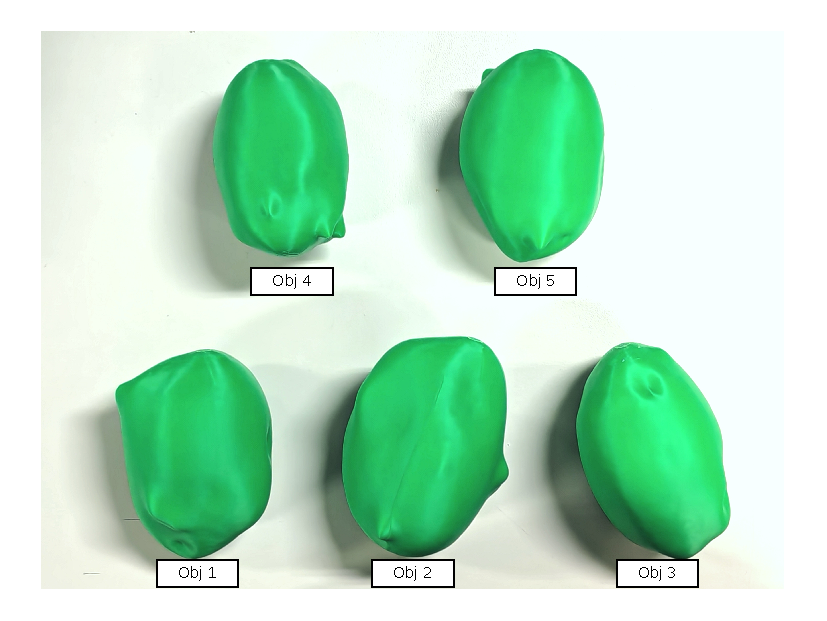
\includegraphics[width=0.8\linewidth]{fig/chp3/chp3_random_potato.drawio.pdf}
    \caption{The 3D-Printed objects used in experiment section \ref{sec:system:pointcloud:evaluation:bottom-surface}.}
    \label{fig:system:pointcloud:evaluation:bottom-surface}
\end{figure}
評価対象は，図\ref{fig:system:pointcloud:evaluation:bottom-surface}に示した，3Dプリンタで作製した5種類の物体である．
真値形状には各物体のCADモデルを用い，ICP位置合わせ後に各点からCADモデルまでの最短距離を計算した．
評価指標は，距離誤差の平均値，標準偏差，およびRMSEである．

\paragraph{結果と考察}

表\ref{tab:system:bottom-pointcloud}に底面点群を含めて取得したモデルの距離誤差を示す．

\begin{table}[t]
  \centering
  \caption{Distance errors of point clouds including bottom-surface acquisition for each object in figure.\ref{fig:system:pointcloud:evaluation:bottom-surface}.}
  \label{tab:system:bottom-pointcloud}
  \small
  \begin{tabular}{lrrr}
    \toprule
    \textbf{Object} & \textbf{Avg. [mm]} & \textbf{Std. [mm]} & \textbf{RMSE [mm]} \\
    \midrule
    Obj 1 & 4.769 & 3.056 & 5.715 \\
    Obj 2 & 4.890 & 3.567 & 6.091 \\
    Obj 3 & 5.095 & 4.446 & 6.768 \\
    Obj 4 & 5.238 & 3.419 & 6.327 \\
    Obj 5 & 4.910 & 4.673 & 6.789 \\
    \bottomrule
  \end{tabular}
\end{table}

5物体の平均距離誤差は4.98\,mm，平均RMSEは6.34\,mmであった．
物体間で平均誤差の差は小さく，最小値はObj 1の4.769\,mm，最大値はObj 4の5.238\,mmであった．
このことから，提案した底面点群取得手順は，対象形状が異なっても同程度の精度で底面側を補完できることが分かる．
一方，表面形状誤差の評価（表\ref{tab:system:container-surface-error}）と比較すると，底面点群を含む場合のRMSEは大きい．
この増加には，持ち上げ時の把持による対象物姿勢の微小変化，ハンド点群除去時の残留点，手指遮蔽による局所的欠損，および持ち上げ姿勢からテーブル上姿勢へ復元する際のロボット手先姿勢誤差が影響していると考えられる．

それでも，底面点群を取得する意義は大きい．
卓上撮影だけでは，底面側は完全に欠落し，点群モデルは上面および側面に偏った開いた形状となる．
これに対して，本手法では把持・持ち上げ・再撮影を用いることで，底面および下部側面を含む閉じた外形に近い点群を得ることができる．
この情報は，物体の幾何学的重心の近似，把持候補点の生成，および安定把持における接触可能領域の評価に有効である．
したがって，底面取得では局所的な誤差は増加するものの，対象物全体の幾何情報を補完するという目的に対しては有効であると考えられる．

\subsection{本セクションのまとめ}

以上の三種類の評価実験から，提案した3D点群モデル取得パイプラインは，標準物体に対しては半径1\,mm未満，位置1--2\,mm程度の誤差で幾何プリミティブを推定できることが確認された．
また，3Dプリンタ製容器に対しては，平均相対誤差2.31\%で容積を推定でき，CADモデルに対する表面RMSEは1.424--3.522\,mmであった．
底面点群取得では，RMSEが5.715--6.789\,mmと大きくなるものの，卓上撮影では取得できない底面側の幾何情報を補完できることを確認した．
これらの結果は，本章で構築した点群取得・処理パイプラインが，後続章の皮むき，注ぎ，および安定把持に必要な幾何情報を提供できることを示している．

\section{まとめ}
\label{sec:system:summary}

本章では，本論文におけるロボットシステムの構成と3D点群モデル取得の共通処理パイプラインについて述べた．
本章の主要な内容を以下に要約する：

\begin{enumerate}
  \item \textbf{ロボットシステムの構成}：双腕ロボット（PA10-7C / DENSO VS-050），力覚センサ，平行グリッパ，RGB-Dカメラからなるハードウェア基盤を構築した．また，三つのタスクそれぞれに適切なエンドエフェクタを設計・実装した．

  \item \textbf{点群取得}：RGB-Dカメラを用いた多視点点群撮影，座標系定義（世界・カメラ・手先の3階層），Hand-Eyeキャリブレーションによる外部パラメータ同定，座標変換による多視点点群合成の手順を確立した．これにより，単一視点では不可視となる領域を含む全周的な物体形状の取得が可能となった．

  \item \textbf{点群処理}：作業領域切り出し，Voxel Gridダウンサンプリング，RANSACによる平面除去，Statistical/Radius Outlier Removalによる外れ値除去，Euclidean Clusteringによる対象物抽出，MLS平滑化と法線ベクトル推定からなる標準処理パイプラインを構築した．これにより，ノイズや作業台平面を除外した高品質な物体点群モデルが得られることを確認した．

  \item \textbf{基礎情報の抽出}：前処理後の点群モデルから，位置姿勢（AABB），色情報，法線ベクトル，断面積と体積（Quickhull凸包＋断面積分），重心，表面領域と指先位置候補を抽出する手法を示した．これらの情報は，後続章における液体注ぎ制御，食材把持位置探索，皮むき軌道生成の基盤となる．

  \item \textbf{底面点群の取得}：机上スキャンで不可視となる底面情報を，把持による持ち上げと再撮影により取得する手法を提案した．さらに，手指遮蔽を低減するためにハンドを$z$軸周りに90$^{\circ}$回転させて再撮影する手順を導入し，底面を含む外形点群を構成できることを確認した．

  \item \textbf{精度評価}：標準物体，3Dプリンタ製容器，および底面点群取得の評価実験により，点群取得・処理パイプラインの実用的な精度を確認した．円柱標準物体では半径誤差が全条件平均で$-0.716\pm0.175$\,mmであり，3Dプリンタ製容器では容積推定の平均相対誤差が2.31\%，CADモデルに対する表面RMSEが1.424--3.522\,mmであった．底面点群を含むモデルではRMSEが5.715--6.789\,mmとなり，底面補完に伴う誤差増加と全体形状補完の効果を確認した．
\end{enumerate}

\begin{revisionblock}
以上の結果から，本章で構築したロボットシステムと点群取得・処理パイプラインは，後続章の三タスクについて必要な幾何情報を供給できることを確認した．
ただし，RGB-D計測には反射・透明表面や遮蔽による欠測があり，底面を含むモデルでは誤差も増加するため，本結果から物体操作一般に対する十分な精度または汎用性を主張するものではない．
家庭用システムへの展開には，装置の小型化，計測時間の短縮，およびキッチンに存在する反射・透明物体に対する追加のロバスト化が必要である．
\end{revisionblock}
